%\documentclass[10pt,times,twocolumn]{paper}
\documentclass[english,aps,prd,nofootinbib,twocolumn]{revtex4-1}
%\documentclass[english,aps,prd,nofootinbib]{revtex4-1}
%\documentclass[twocolumn,english,aps,prd,nofootinbib]{revtex4-1}
\usepackage{CJK}

%\usepackage{tikz}
\usepackage{amsfonts}
\usepackage{amsmath}
\usepackage{hyperref}
\usepackage{amssymb}
\usepackage{mathtools}
\usepackage{cleveref}
\usepackage{cancel}
\usepackage{xfrac}
\usepackage{xcolor}
\usepackage{relsize}%\mathlarger command 
%\usetikzlibrary{arrows,decorations.markings}
\usepackage[bottom]{footmisc}

%\usepackage{newtxtext}
%\usepackage{multicol}
%\usepackage{comment}
\usepackage{tikz}
\usepackage{tikz-feynman}
\usetikzlibrary{calc,arrows,decorations.markings,snakes,shapes}
\usepackage{pgfplots}
\pgfplotsset{compat=1.3}
\usetikzlibrary{3d,calc}

\newcommand{\largepentagon}{\large{\pentagon}}
\newcommand{\largevarhexagon}{\large{\varhexagon}}

\newcommand{\tstar}[5]{% inner radius, outer radius, tips, rot angle, options
\pgfmathsetmacro{\starangle}{360/#3}
\draw[#5] (#4:#1)
\foreach \x in {1,...,#3}
{ -- (#4+\x*\starangle-\starangle/2:#2) -- (#4+\x*\starangle:#1)
}
-- cycle;
}

\newcommand{\ngram}[4]{% outer radius, tips, rot angle, options
\pgfmathsetmacro{\starangle}{360/#2}
\pgfmathsetmacro{\innerradius}{#1*sin(90-\starangle)/sin(90+\starangle/2)}
\tstar{\innerradius}{#1}{#2}{#3}{#4}
}

%\usepackage{subfigure}
%\usepackage{subcaption}
%\captionsetup[subfigure]{labelformat=brace}

%\usetikzlibrary{tikzmark,fit}

\usepackage{units}

%%%%%%%%%%%%%%%%%%%%%%%%%%%%%%%%%%%%%%%%%%%%%%%%%%%%%%%%%%

\newcommand{\sfms}[1]{\textbf{\textcolor{blue}{(#1 --Seb)}}}
\newcommand{\inti}[1]{\textbf{\textcolor{green}{(#1 --El Jefe)}}}

\renewcommand{\textfraction}{0.10}
\renewcommand{\topfraction}{0.90}
\renewcommand{\bottomfraction}{0.90}
\renewcommand{\floatpagefraction}{0.65}

\usepackage{xspace}



%%%%%%%%%%%%%%%%%%%%%%%%%%%%%%%%%%%%%%%%%%%%%%%%%%%%%%%%%%

\usepackage{color}
\usepackage{graphicx}
\usepackage[space]{grffile}
%\usepackage{indentfirst}
\usepackage{verbatim}
\usepackage{amsmath}
\usepackage{amssymb}
\usepackage{wasysym}%pentagons, hexagons, octagons
\usepackage{ifsym}%
\usepackage[caption=false]{subfig}
\usepackage{url}
\usepackage{bbold}
\usepackage{slashed}
\usepackage{epstopdf}
\usepackage{braket}
\usepackage{float}

%\usepackage{biblatex}

\newcommand{\aaps}{{Astron.~Astrophys.~Supp.}}
\newcommand{\physrep}{{Physics~Reports}}
\newcommand{\araa}{{Annu.~Rev.~Astron.~Astrophys.}}
\newcommand{\aap}{{Astron.~Astrophys.}}
\newcommand{\apjl}{{Astrophys.~J.~Lett.}}
\newcommand{\apjs}{{Astrophys.~J.~Supp.}}
\newcommand{\aj}{{Astron.~J.}}
%\newcommand{\apj}{The Astrophysics Journal}
\newcommand{\mnras}{{Mon.~Not.~R.~Astron.~Soc.}}
\newcommand{\aapr}{{Astronomy and Astrophysics Reviews}}

\DeclareRobustCommand{\Sec}[1]{Sec.~\ref{#1}}
\DeclareRobustCommand{\Secs}[2]{Secs.~\ref{#1} and \ref{#2}}
\DeclareRobustCommand{\App}[1]{App.~\ref{#1}}
\DeclareRobustCommand{\Tab}[1]{Table~\ref{#1}}
\DeclareRobustCommand{\Tabs}[2]{Tables~\ref{#1} and \ref{#2}}
\DeclareRobustCommand{\Fig}[1]{Fig.~\ref{#1}}
\DeclareRobustCommand{\Figs}[2]{Figs.~\ref{#1} and \ref{#2}}
\DeclareRobustCommand{\Eq}[1]{Eq.~(\ref{#1})}
\DeclareRobustCommand{\Eqs}[2]{Eqs.~(\ref{#1}) and (\ref{#2})}
\DeclareRobustCommand{\Ref}[1]{Ref.~\cite{#1}}
\DeclareRobustCommand{\Refs}[1]{Refs.~\cite{#1}}
\DeclareMathAlphabet\mathbfcal{OMS}{cmsy}{b}{n}

\newcommand{\boundellipse}[3]% center, xdim, ydim
{[black,fill=blue!30] (#1) ellipse (#2 and #3)
}
\newcommand{\boundellipseW}[3]% center, xdim, ydim
{[white,fill=white] (#1) ellipse (#2 and #3)
}
\newcommand*{\Scale}[2][4]{\scalebox{#1}{$#2$}}%
\newcommand*{\Resize}[2]{\resizebox{#1}{!}{$#2$}}%
\DeclareMathOperator*{\Motimes}{\text{\raisebox{0.25ex}{\scalebox{0.8}{$\bigotimes$}}}}
%\usepackage{mathabx,graphicx}
\def\Circlearrowleft{\ensuremath{%
  \rotatebox[origin=c]{180}{$\circlearrowleft$}}}
\def\Circlearrowright{\ensuremath{%
  \rotatebox[origin=c]{180}{$\circlearrowright$}}}
\def\CircleArrowleft{\ensuremath{%
  \reflectbox{\rotatebox[origin=c]{180}{$\circlearrowleft$}}}}
\def\CircleArrowright{\ensuremath{%
  \reflectbox{\rotatebox[origin=c]{180}{$\circlearrowright$}}}}
  
\newcounter{countitems}
\newcounter{nextitemizecount}
\newcommand{\setupcountitems}{%
  \stepcounter{nextitemizecount}%
  \setcounter{countitems}{0}%
  \preto\item{\stepcounter{countitems}}%
}
\makeatletter
\newcommand{\computecountitems}{%
  \edef\@currentlabel{\number\c@countitems}%
  \label{countitems@\number\numexpr\value{nextitemizecount}-1\relax}%
}
\newcommand{\nextitemizecount}{%
  \getrefnumber{countitems@\number\c@nextitemizecount}%
}
\newcommand{\previtemizecount}{%
  \getrefnumber{countitems@\number\numexpr\value{nextitemizecount}-1\relax}%
}
\makeatother    
\newenvironment{AutoMultiColItemize}{%
\ifnumcomp{\nextitemizecount}{>}{3}{\begin{multicols}{2}}{}%
\setupcountitems\begin{itemize}}%
{\end{itemize}%
\unskip\computecountitems\ifnumcomp{\previtemizecount}{>}{3}{\end{multicols}}{}}


\hyphenation{dia-go-na-li-za-tion}

\begin{document}

\title{Multilayer graphene}

%\author{Sebastian Mantilla$^{1}$}
%\email{mantilla@pks.mpg.de}
%\author{Inti Sodemann$^{1}$}
%\email{sodemann@pks.mpg.de}


%\affiliation{$^1$Department of Physics, Princeton University, Princeton, NJ 08544}

%\affiliation{$^1$Max-Planck Institute for the Physics of Complex Systems, D-01187 Dresden, Germany}

%\date{\today}


%\maketitle	

\section*{Multilayer graphene}

%\tableofcontents



%\begin{abstract}
%We develop a bosonization formalism that captures non-perturbatively the interaction effects on the $\mathbf{Q}=0$ continuum of excitations of nodal fermions above one dimension. Our approach is a natural extension of the classic bosonization scheme for higher dimensional Fermi surfaces 
%~\cite{luther1979tomonaga, haldane2005luttinger, houghton1993bosonization, neto1994bosonization} 
%to include the $\mathbf{Q}=0$ neutral excitations that would be absent in a single-band system. The problem is reduced to solving a boson bilinear Hamiltonian. We establish a rigorous microscopic footing for this approach by showing that the solution of such boson bilinear Hamiltonian is exactly equivalent to performing the infinite sum of Feynman diagrams associated with the Kadanoff-Baym particle-hole propagator that arises from the self-consistent Hartree-Fock approximation to the single particle Green's function. We apply this machinery to compute the interaction corrections to the optical conductivity of 2D Dirac Fermions with Coulomb interactions reproducing the results of perturbative renormalization group at weak coupling and extending them to the strong coupling regime. 
%\end{abstract}


\section{Scales of the Hamiltonian}
We set $\hbar = 1$ throughout all the text. The UV cutoff $\mathcal{K}$ of the system, fixed by the lattice parameter $2\pi/\mathcal{K}$, provides us a natural scale to measure the momenta, such that any momentum index $\mathbf{k}$ is normalized by $\mathcal{K}$. In this way, we get the kinetic non-interacting Hamiltonian
\begin{equation}
\label{eq:Main-Ham}
\begin{split}
&H_{\mathrm{kin}} = 
E_{\mathrm{UV} }\sum_{\mathbf{k }\sigma\sigma'}
\left(\frac{|\mathbf{k}|}{\mathcal{K}}\right)^{m}
\psi_{\mathbf{k },\sigma}^{\textcolor{black}{\dagger}}
\left( \hat{\mathbf{k}}_{m} \cdot 
\boldsymbol{\sigma}_{\sigma\sigma'} \right)
\psi_{\mathbf{k },\sigma'}^{\textcolor{white}{\dagger}}
,
\end{split}
\end{equation}
where $[\hat{\mathbf{k}}_{m}]= 
\begin{pmatrix}
\cos(m\phi_{m})	&	\!\!\sin(m\phi_{m})
\end{pmatrix}$ and $E_{\mathrm{UV} }$ is the numerical value of the kinetic term evaluated at $\mathcal{K}$, and whose shape depends on $m$:
\begin{itemize}
\item $m=1$: $E_{\mathrm{UV} } = v\mathcal{K}$, where $v$ is the Fermi velocity of the Dirac fermions.
\item $m=2$: $E_{\mathrm{UV} } = \mathcal{K}^{2}/2m_{e}$, where $m_{e}$ is the effective mass of the electron. 
\end{itemize}
Therefore, the density of states per spin and per valley can be expressed as
\begin{equation}
N(E) = \frac{\mathcal{K}^{2}}{2\pi m}
\sqrt[m]{
\frac{E^{2-m}_{\textcolor{white}{b}}}
{E_{\mathrm{UV}}^{2}}},
\end{equation}
which, as special cases:
\begin{itemize}
\item $m=1$: $N(E)\propto (\mathcal{K}/E_{\mathrm{UV}})^{2}E=E/ v^{2}$.
\item $m=2$: $N(E)\propto \mathcal{K}^{2}/E_{\mathrm{UV}}=2m_{e}$.
\end{itemize}
On the other hand, the interaction Hamiltonian can be expressed as
\begin{eqnarray}
&H&\!_{\mathrm{int}} =
\frac{1}{2A}
%\sum_{\genfrac{ }{ }{0pt}{3}{\mathbf{k },\mathbf{k'}}{\mathbf{q }\neq 0} } 
\sum_{\mathbf{k }\mathbf{k'}}
\sum_{\sigma \sigma'} 
V_{\mathbf{q}}
\psi_{\mathbf{k'+q,\sigma'}}^{\textcolor{black}{\dagger}}
\psi_{\mathbf{k -q,\sigma }}^{\textcolor{black}{\dagger}}
\psi_{\mathbf{k   ,\sigma }}^{\textcolor{white}{\dagger}}
\psi_{\mathbf{k'  ,\sigma'}}^{\textcolor{white}{\dagger}},
\end{eqnarray}
where $A$ is the total area of the system.

\section{Restricted Hilbert space for $\mathbf{Q}=0$ excitons and pseudospin basis}

The optical relevant excitations of the system correspond to the $\mathbf{Q}=0$ excitons, as shown in Fig. \ref{fig:Q=0-excitons}. These ones do not modify the momentum label of the electron when it jumps from the valence to the conduction band, and consequently, any interaction between a pair excitons at momenta $\mathbf{k}_{1}$ and $\mathbf{k}_{2}$ should only interchange their momentum labels. In other words, by having into account only $\mathbf{Q}=0$ excitations, the Hilbert space of the system results restricted onto the singly-occupied sites in the momentum lattice. A good operator to describe the singly-occupied constrain is
\begin{equation}
\label{eq:SU(2)-spin-operator}
s^{\mu}_{\mathbf{k }} = \sum_{\sigma \sigma'} 
\psi_{\mathbf{k ,\sigma }}^{\textcolor{black}{\dagger}}
\sigma^{\mu }_{\sigma \sigma'}
\psi_{\mathbf{k ,\sigma'}}^{\textcolor{white}{\dagger}}.
\end{equation}
where $\sigma^{\mu }_{\sigma  ,\sigma '}$ is the component $\sigma \sigma '$ of the matrix $\sigma^{\mu }$, given by the generators ot the SU(2) Lie algebra, i.e., the Pauli matrices and the identity
\begin{equation}
\begin{matrix}
\sigma^{0}_{\textcolor{white}{,}} = 
\begin{pmatrix}
1	&	0	\\	0	&	1
\end{pmatrix}	&	,	&	
\sigma^{1}_{\textcolor{white}{,}} = 
\begin{pmatrix}
0	&	1	\\	1	&	0
\end{pmatrix}	&	, \\
\sigma^{2}_{\textcolor{white}{,}} = 
\begin{pmatrix}
0	&	-i	\\	i	&	0
\end{pmatrix}	&	,	&	
\sigma^{3}_{\textcolor{white}{,}} = 
\begin{pmatrix}
1	&	0	\\	0	&	-1
\end{pmatrix}	&	,
\end{matrix}
\end{equation}
The matrix $\sigma^{0}$ is useful to express the singly-occupied condition as the constrain
\begin{equation}
\begin{split}
s^{0}_{\mathbf{k }} &= \sum_{\sigma \sigma'} 
\psi_{\mathbf{k ,\sigma }}^{\textcolor{black}{\dagger}}
\sigma^{0}_{\sigma \sigma'}
\psi_{\mathbf{k ,\sigma'}}^{\textcolor{white}{\dagger}} =
\sum_{\sigma \sigma'} 
\psi_{\mathbf{k ,\sigma }}^{\textcolor{black}{\dagger}}
\delta_{\sigma \sigma'}
\psi_{\mathbf{k ,\sigma'}}^{\textcolor{white}{\dagger}} \\ &=
\sum_{\sigma \sigma'} 
\psi_{\mathbf{k ,\sigma }}^{\textcolor{black}{\dagger}}
\psi_{\mathbf{k ,\sigma }}^{\textcolor{white}{\dagger}} =
\sum_{\sigma } 
n_{\mathbf{k ,\sigma }} = 
1.
\end{split}
\end{equation}.

\begin{figure}
\centering
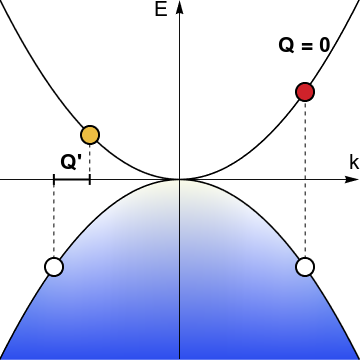
\includegraphics[scale=0.45]{ParabolicVertical.png}
\caption{$\mathbf{Q}=0$ and $\mathbf{Q}\neq 0$ excitations on the parabolic bands.}
\label{fig:Q=0-excitons}
\end{figure}

The following steps show how the four-fermion term in the interacion Hamiltonian can be expressed under the singly-occupied constrain. The completeness relation of the Pauli matrices
\begin{equation}
\sum_{\mu=0}^{3} 
\sigma^{\mu }_{\sigma \sigma'}\sigma^{\mu }_{\tau \tau'} =  
2 \delta_{\sigma \tau'} \delta_{\sigma'\tau },
\end{equation}
and the trace of Pauli matrices bilinears 
\begin{equation}
\mathrm{tr}\left( \sigma^{\mu }\sigma^{\mu'} \right) = 
\sum_{\tau ,\tau'}
\sigma^{\mu }_{\tau \tau'}\sigma^{\mu'}_{\tau'\tau } = 
2 \delta^{\mu \mu'},
\end{equation}
are useful to find the inverse relation between fermion bilinears and Pauli matrices
\begin{equation}
\begin{split}
\sum_{\mu=0}^{3} 
\sigma^{\mu }_{\tau \tau'}s^{\mu}_{\mathbf{k }} &= 
\sum_{\mu=0}^{3} \sum_{\sigma \sigma'} 
\psi_{\mathbf{k ,\sigma }}^{\textcolor{black}{\dagger}}
\sigma^{\mu }_{\sigma \sigma'}\sigma^{\mu }_{\tau ,\tau'}
\psi_{\mathbf{k ,\sigma'}}^{\textcolor{white}{\dagger}} \\ &= 
2
\sum_{\sigma \sigma'} 
\psi_{\mathbf{k ,\sigma }}^{\textcolor{black}{\dagger}}
\delta_{\sigma \tau'} \delta_{\sigma'\tau }
\psi_{\mathbf{k ,\sigma'}}^{\textcolor{white}{\dagger}} \\ &= 
2
\psi_{\mathbf{k ,\tau'}}^{\textcolor{black}{\dagger}}
\psi_{\mathbf{k ,\tau }}^{\textcolor{white}{\dagger}} .
\end{split}
\end{equation}
In this way, the fermion bilinears can then be expanded in terms of the generators of the Lie algebra of the group $\mathrm{SU}(2)$
\begin{equation}
\label{eq:SU(2)-expansion-of-fermion-bilinears}
\psi_{\mathbf{k ,\tau'}}^{\textcolor{black}{\dagger}}
\psi_{\mathbf{k ,\tau }}^{\textcolor{white}{\dagger}} = 
\frac{1}{2}
\sum_{\mu=0}^{3} 
s^{\mu }_{\mathbf{k }}\sigma^{\mu }_{\tau \tau'},
\end{equation}

The Eq. \eqref{eq:SU(2)-expansion-of-fermion-bilinears}
is then useful to express the four-fermion term of the interaction Hamiltonian after some anticommutations to match fermion operators that share the same momentum label, such as follows
\begin{equation}
\begin{split}
\sum_{\tau ,\tau'}&
\left(\psi_{\mathbf{k ,\tau   }}^{\textcolor{black}{\dagger}}
\psi_{\mathbf{k ,\tau'  }}^{\textcolor{white}{\dagger}}\right)
\left(\psi_{\mathbf{k',\sigma }}^{\textcolor{black}{\dagger}}
\psi_{\mathbf{k',\sigma'}}^{\textcolor{white}{\dagger}}\right)
 = \\ &=
\sum_{\tau ,\tau'}
\left(
\frac{1}{2} 
\sum_{\mu =0}^{3} 
\sigma^{\mu }_{\tau'\tau }s^{\mu }_{\mathbf{k }}
\right)
\left(
\frac{1}{2} 
\sum_{\mu'=0}^{3} 
\sigma^{\mu'}_{\tau \tau'}s^{\mu'}_{\mathbf{k'}}
\right) \\ &=
\frac{1}{4}
\sum_{\mu ,\mu'}
s^{\mu }_{\mathbf{k }}
s^{\mu'}_{\mathbf{k'}}
\sum_{\tau ,\tau'}
\sigma^{\mu }_{\tau'\tau }
\sigma^{\mu'}_{\tau \tau'}
 \\ &=
\frac{1}{4}
\sum_{\mu ,\mu'}
s^{\mu }_{\mathbf{k }}
s^{\mu'}_{\mathbf{k'}}
\mathrm{tr}\left( \sigma^{\mu }\sigma^{\mu'} \right)
\\ &=
\frac{1}{2}
\sum_{\mu ,\mu'}
s^{\mu }_{\mathbf{k }}
s^{\mu'}_{\mathbf{k'}}
\delta^{\mu \mu'}
=
\frac{1}{2}
\sum_{\mu ,\mu'}
s^{\mu }_{\mathbf{k }}
s^{\mu }_{\mathbf{k'}}
=
\frac{
1 + 
\mathbf{s}_{\mathbf{k }}
\cdot
\mathbf{s}_{\mathbf{k'}}
}{2}
\end{split}
\end{equation}

Consequently, the original fermion Hamiltonian projected onto the singly-occupied is expressed as
\begin{equation}
\label{eq:Effective-Heisenberg-Hamiltonian}
\begin{split}
\mathcal{P} H \mathcal{P} &= \\
E_{\mathrm{UV} }&
\sum_{\mathbf{k }} \left(\frac{|\mathbf{k}|}{\mathcal{K}}\right)^{m}
\!\! 
\hat{\mathbf{k}}_{m}\!\! \cdot \mathbf{s}_{\mathbf{k }} - 
\sum_{\mathbf{k}_{1} \neq \mathbf{k}_{2}}
%\overbrace{
\frac{V_{\mathbf{k}_{1}-\mathbf{k}_{2}}}{4A}
\mathbf{s}_{\mathbf{k}_{1}}\!\!
\cdot
\mathbf{s}_{\mathbf{k}_{2}}
,
\end{split}
%}^{Ferromag.\;exchange}
\end{equation}
where the first term represents a $m$-folded spin vortex (see Fig. \ref{fig:Classical-gound-state}) and the second term is an effective ferromagnetic exchange. 

\section{Expansion about the non-interacting ground state}


\subsection{Band basis and interaction matrix}
\label{sect:Supp:Band-basis}

\begin{figure}
\centering
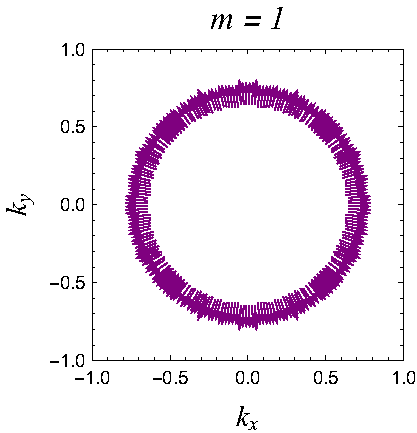
\includegraphics[scale=0.6]{1Layer.pdf}
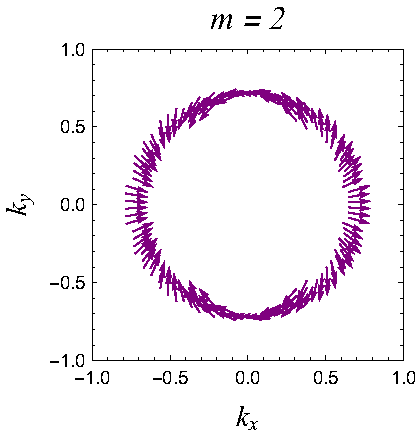
\includegraphics[scale=0.6]{2Layer.pdf}
%\includegraphics[scale=0.8]{3Layer.pdf}
%\includegraphics[scale=0.8]{4Layer.pdf}
%\includegraphics[scale=0.8]{5Layer.pdf}
%\includegraphics[scale=0.8]{6Layer.pdf}
\caption{Polar distribution of the vector $[\hat{\mathbf{k}}_{m}]= 
\begin{pmatrix}
\cos(m\phi_{m})	&	\!\!\sin(m\phi_{m})
\end{pmatrix}$ used to describe the classical ground state of the system.}
\label{fig:Classical-gound-state}
\end{figure}

In this section, we provide details of the derivation of Eqs. \eqref{eq:HP-Hamiltonian} to \eqref{eq:Interacion-matrix} starting from Eq. \eqref{eq:Main-Ham}. We begin describing the transfomation from pseudo-spin basis onto band basis. In the band basis $s=\{+,-\}$ the kinetic term is:
\begin{equation}
\begin{split}
\psi_{\mathbf{k }\sigma }^{\textcolor{black}{\dagger}}&
\left( \hat{\mathbf{k}}_{m} \cdot 
\boldsymbol{\sigma}_{\sigma\sigma'} \right)
\psi_{\mathbf{k }\sigma'}^{\textcolor{white}{\dagger}}
 = 
\\ &= 
    e^{-im\phi}
    \psi_{\mathbf{k\uparrow  }}^{\textcolor{black}{\dagger}}
    \psi_{\mathbf{k\downarrow}}^{\textcolor{white}{\dagger}} + 
    e^{+im\phi}
    \psi_{\mathbf{k\downarrow}}^{\textcolor{black}{\dagger}}
    \psi_{\mathbf{k\uparrow  }}^{\textcolor{white}{\dagger}} 
    .
\end{split}
\end{equation}
Band and pseudospin basis are related by:
\begin{equation}
\begin{split}
	\psi_{\mathbf{k}\sigma} &= 
	\sum_{s}
	\left\langle \sigma | \mathbf{k }s \right\rangle
	\psi_{\mathbf{k} s },	\\
\begin{pmatrix}
    \psi_{\mathbf{k\uparrow  }}	\\
    \psi_{\mathbf{k\downarrow}}	
\end{pmatrix} &= 
\frac{1}{\sqrt{2}}
\begin{pmatrix}
	 e^{- im\phi /2}	& 
	 e^{- im\phi /2}	\\  
	 e^{+ im\phi /2}	&
    -e^{+ im\phi /2}
\end{pmatrix}
\begin{pmatrix}
	\psi_{\mathbf{k+}}	\\
	\psi_{\mathbf{k-}}	
\end{pmatrix}.
\end{split}
\end{equation}
Fermion bilinears transform as
\begin{equation}
\begin{split}
\sum_{\sigma}
\psi_{\mathbf{k}_{1}\sigma}^{\textcolor{black}{\dagger}}
\psi_{\mathbf{k}_{2}\sigma}^{\textcolor{white}{\dagger}}
&= 
\psi_{\mathbf{k}_{1}s_{1} }^{\textcolor{black}{\dagger}}
\sum_{s_{1}s_{2}}\!\!
\left\langle \mathbf{k}_{1}s_{1} | \mathbf{k}_{2}s_{2} \right\rangle \psi_{\mathbf{k}_{1}s_{1} }^{\textcolor{black}{\dagger}}
\psi_{\mathbf{k}_{2}s_{2} }^{\textcolor{white}{\dagger}},
\end{split}
\end{equation}
where
\begin{equation}
\begin{split}
& \left\langle \mathbf{k}_{1}s_{1} | \mathbf{k}_{2}s_{2} \right\rangle =
\begin{pmatrix}
     \cos\sfrac{m\phi_{12}}{2}  &    i\sin\sfrac{m\phi_{12}}{2} \\  
    i\sin\sfrac{m\phi_{12}}{2}  &     \cos\sfrac{m\phi_{12}}{2}
\end{pmatrix},
\end{split}
\end{equation}
where $\phi_i$ is the polar angle of $\mathbf{k}_i$, and  $\phi_{12}=\phi_1-\phi_2$. Therefore, the Hamiltonian in Eq. \eqref{eq:Main-Ham} of the Main text in the band basis is expressed as follows:
\begin{equation}
\begin{split}
&\mathcal{P} H \mathcal{P} = 
\sum_{\mathbf{k }}E^{m}_{\mathbf{k}}
\left( 
\psi_{\mathbf{k}+ }^{\textcolor{black}{\dagger}}
\psi_{\mathbf{k}+ }^{\textcolor{white}{\dagger}} - 
\psi_{\mathbf{k}- }^{\textcolor{black}{\dagger}}
\psi_{\mathbf{k}- }^{\textcolor{white}{\dagger}}
\right)
\\
&- 
\sum_{\mathbf{k}_{1}\neq \mathbf{k}_{2}} 
\sum_{s_{1} s_{2}} 
(T^{m}_{\mathbf{k}_{1}\mathbf{k}_{2}})^{s_{1}s_{2}}
\psi_{\mathbf{k}_{1}s_{1} }^{\textcolor{black}{\dagger}}
\psi_{\mathbf{k}_{1}\bar{s}_{1} }^{\textcolor{white}{\dagger}}
\psi_{\mathbf{k}_{2}\bar{s}_{2} }^{\textcolor{black}{\dagger}}
\psi_{\mathbf{k}_{2}s_{2} }^{\textcolor{white}{\dagger}}
,
\end{split}
\end{equation}
where $E^{m}_{\mathbf{k}}=E_{\mathrm{UV} }(|\mathbf{k}|/\mathcal{K})^{m}+\Sigma^{m}_{\mathbf{k}}$ is the effective dispersion relation of the electrons, in which $\Sigma^{m}_{\mathbf{k}}$ is the self-energy
\begin{eqnarray}
\label{eq:Supp:Self-Energy-expression}
\begin{split}
\Sigma^{m}_{\mathbf{k }} = 
\frac{1}{2A}\sum_{\mathbf{p}}V_{\mathbf{k-p}}\cos(m\phi_{\mathbf{kp}}).
\end{split}
\end{eqnarray}
and $(T^{m})_{\mathbf{k}_{1}\mathbf{k}_{2}}^{s_{1}s_{2}}$ is the interaction matrix in the band basis, given by:
\begin{equation}
\label{eq:Supp:Interaction-matrix-band-basis}
T^{m}_{\mathbf{k}_{1}\mathbf{k}_{2}} \! = \!
\frac{V_{\mathbf{k_{1}-k_{2}}}}{4A} 
\begin{pmatrix}
    1+\cos(m\phi_{12})  &    1-\cos(m\phi_{12}) \\  
    1-\cos(m\phi_{12})  &    1+\cos(m\phi_{12})
\end{pmatrix}.
\end{equation}

\subsection{Holstein-Primakoff expansion}
\label{sect:Supp:Holstein-Primakoff}
We select the following spin basis 
\begin{equation}
\label{eq:Supp:Zeemann-basis}
\mathbf{s}_{\mathbf{k}} = -
s_{\mathbf{k}}^{z}\hat{\mathbf{k}}_{m} + 
s_{\mathbf{k}}^{x} \hat{\mathbf{z}} + 
s_{\mathbf{k}}^{y}\hat{\boldsymbol{\phi}}_{m},
\end{equation}
which diagonalizes the kinetic term, and where $\hat{\mathbf{z}}$ is the normal axis to the layer and $\hat{\boldsymbol{\phi}}_{m}=\hat{\mathbf{z}}\times \hat{\mathbf{k}}_{m} = 
\begin{pmatrix}
-\sin(m\phi_{m})	&	\!\!\cos(m\phi_{m})
\end{pmatrix}$, and the exchange term is expanded as
\begin{eqnarray}
\label{eq:Spin-dot-product-along-k}
\hat{\mathbf{s}}_{\mathbf{k}}\!\! &\cdot& \hat{\mathbf{s}}_{\mathbf{k}'} 
\\ &=& \nonumber 
\left( -\hat{s}_{\mathbf{k}_{1}}^{z} \hat{\mathbf{k}} + \hat{s}_{\mathbf{k }}^{x} \hat{\mathbf{z }} + \hat{s}_{\mathbf{k }}^{y} \hat{\boldsymbol{\varphi}} \right) \cdot \left( -\hat{s}_{\mathbf{k'}}^{z} \hat{\mathbf{k'}} + \hat{s}_{\mathbf{k'}}^{x} \hat{\mathbf{z }} + \hat{s}_{\mathbf{k'}}^{y} \hat{\boldsymbol{\varphi}}'\right) 
\\ &=& \nonumber 
\left(
\hat{s}_{\mathbf{k }}^{z}\hat{s}_{\mathbf{k'}}^{z}+ \hat{s}_{\mathbf{k }}^{y}\hat{s}_{\mathbf{k'}}^{y} \right)\cos \phi_{\mathbf{k}\mathbf{k'}} + 
\hat{s}_{\mathbf{k }}^{x}\hat{s}_{\mathbf{k'}}^{x} 
\\ &+& \,
\left(
\hat{s}_{\mathbf{k }}^{y}\hat{s}_{\mathbf{k'}}^{z}- \hat{s}_{\mathbf{k }}^{z}\hat{s}_{\mathbf{k'}}^{y} \right)\sin \phi_{\mathbf{k}\mathbf{k'}}
\nonumber	
\end{eqnarray}
with $\cos \phi_{\mathbf{k}\mathbf{k'}} = \hat{\mathbf{k }}\cdot\hat{\mathbf{k'}} = \hat{\boldsymbol{\varphi}}\cdot\hat{\boldsymbol{\varphi}}'$. 
On this basis, the Hamiltonian can be expanded in a bosonic representation by means of the Holstein-Primakoff (HP) transformations ($S=\nicefrac{1}{2}$):
\begin{equation}
\label{eq:Holstein-Primakoff}
\begin{split}
s_{\mathbf{k }}^{z} &= 2\left( S - 
b_{\mathbf{k }}^{\textcolor{black}{\dagger}}
b_{\mathbf{k }}^{\textcolor{white}{\dagger}} \right) = 1 - 2 
b_{\mathbf{k }}^{\textcolor{black}{\dagger}}
b_{\mathbf{k }}^{\textcolor{white}{\dagger}}
, \\
s_{\mathbf{k }}^{x}  
&\approx \sqrt{2 S}\left( 
b_{\mathbf{k }}^{\textcolor{white}{\dagger}} + 
b_{\mathbf{k }}^{\textcolor{black}{\dagger}} \right) = 
b_{\mathbf{k }}^{\textcolor{white}{\dagger}} + 
b_{\mathbf{k }}^{\textcolor{black}{\dagger}}
, \\
i s_{\mathbf{k }}^{y}
&\approx \sqrt{2 S}\left( 
b_{\mathbf{k }}^{\textcolor{white}{\dagger}} - 
b_{\mathbf{k }}^{\textcolor{black}{\dagger}} \right) = 
b_{\mathbf{k }}^{\textcolor{white}{\dagger}} - 
b_{\mathbf{k }}^{\textcolor{black}{\dagger}}
.
\end{split}
\end{equation}
The term corresponding to the exchange coupling in Eq. \eqref{eq:Effective-Heisenberg-Hamiltonian} can be transformed into pairing and hopping terms of bosons up to bilinears:
\begin{equation}
\begin{split}
\mathbf{s}_{\mathbf{k }} \cdot \mathbf{s}_{\mathbf{k'}} &\approx 
\left(
1+
b_{\mathbf{k }}^{\textcolor{black}{\dagger}}
b_{\mathbf{k }}^{\textcolor{white}{\dagger}} + b_{\mathbf{k'}}^{\textcolor{black}{\dagger}}b_{\mathbf{k'}}^{\textcolor{white}{\dagger}}\right)  
\cos \phi_{\mathbf{k }\mathbf{k'}}
\\ &+ 
\left(
b_{\mathbf{k }}^{\textcolor{black}{\dagger}}
b_{\mathbf{k'}}^{\textcolor{white}{\dagger}} + 
b_{\mathbf{k }}^{\textcolor{white}{\dagger}}
b_{\mathbf{k'}}^{\textcolor{black}{\dagger}}\right) 
\left( 1 + \cos \phi_{\mathbf{k }\mathbf{k'}} \right) 
\\ &+ 
 \left(
b_{\mathbf{k }}^{\textcolor{black}{\dagger}}
b_{\mathbf{k'}}^{\textcolor{black}{\dagger}} + 
b_{\mathbf{k }}^{\textcolor{white}{\dagger}}
b_{\mathbf{k'}}^{\textcolor{white}{\dagger}}
\right) 
\left( 1 - \cos \phi_{\mathbf{k }\mathbf{k'}} \right)
\\ &+ i
 \left(
b_{\mathbf{k }}^{\textcolor{black}{\dagger}} - 
b_{\mathbf{k'}}^{\textcolor{black}{\dagger}} - 
b_{\mathbf{k }}^{\textcolor{white}{\dagger}} +
b_{\mathbf{k'}}^{\textcolor{white}{\dagger}}
\right) 
\sin \phi_{\mathbf{k }\mathbf{k'}}.
\end{split}
\end{equation}

The resulting bosonic Hamiltonian after applying the HP transformations is:
\begin{eqnarray}
\label{eq:Supp:HP-Hamiltonian}
\nonumber && \!\!\!\!\!\!\! 
H_{HP} = \sum_{\mathbf{k}} 
2 E_{\mathrm{UV} }
\left(\frac{|\mathbf{k}|}{\mathcal{K}}\right)^{m} 
\!\!\!
b_{\mathbf{k }}^{\textcolor{black}{\dagger}}
b_{\mathbf{k }}^{\textcolor{white}{\dagger}}
\!
+
\!
\sum_{\mathbf{k}\neq \mathbf{p}}
\frac{V_{\mathbf{k-p}}}{A}
b_{\mathbf{k }}^{\textcolor{black}{\dagger}}
b_{\mathbf{k }}^{\textcolor{white}{\dagger}}
\cos (m\phi_{\mathbf{k }\mathbf{p }})
\\ &+ &
\sum_{\mathbf{k}\neq \mathbf{k'}} 
\!
\frac{V_{\mathbf{k-k'}}}{4A}
\!
\left( 1 + \cos(m\phi_{\mathbf{k}_{1}\mathbf{k}_{2}}) \right) 
\!
\left(	
b_{\mathbf{k}_{1}}^{\textcolor{black}{\dagger}}
b_{\mathbf{k}_{2}}^{\textcolor{white}{\dagger}} + 
b_{\mathbf{k}_{1}}^{\textcolor{white}{\dagger}}
b_{\mathbf{k}_{2}}^{\textcolor{black}{\dagger}}
\right) + 
\\ 
\nonumber &+ &
\sum_{\mathbf{k}\neq \mathbf{k'}} 
\!
\frac{V_{\mathbf{k-k'}}}{4A}
\!
\left( 1 - \cos(m\phi_{\mathbf{k}_{1}\mathbf{k}_{2}}) \right) 
\!
\left(	
b_{\mathbf{k}_{1}}^{\textcolor{black}{\dagger}}
b_{\mathbf{k}_{2}}^{\textcolor{black}{\dagger}} + 
b_{\mathbf{k}_{1}}^{\textcolor{white}{\dagger}}
b_{\mathbf{k}_{2}}^{\textcolor{white}{\dagger}}
\right). 
\end{eqnarray}
The first line contains the kinetic and self-energy terms. The second line can be viewed as boson hopping terms in the momentum lattice. The third line can be viewed as pairing terms which change the number of bosons. Lastly, by using the Bogoliubov basis given by
\begin{equation}
\label{eq:Supp:Bogoliubov-basis}
B^{\dagger}_{\mathbf{k}} = 
\begin{pmatrix}
b^{\textcolor{black}{\dagger}}_{\mathbf{k}}	&	
b^{\textcolor{white}{\dagger}}_{\mathbf{k}}
\end{pmatrix},
\end{equation}
the Hamiltonian can be expressed as 
\begin{equation}
\label{eq:HP-Hamiltonian}
\begin{split}
&H_{HP} = %\sum_{\mathbf{k}} 2v |\mathbf{k }| 
\sum_{\mathbf{k}_{1},\mathbf{k}_{2}} 
B_{\mathbf{k }_{1}}^{\textcolor{black}{\dagger}}
H_{\mathbf{k }_{1}\mathbf{k }_{2}}
B_{\mathbf{k }_{2}}^{\textcolor{white}{\dagger}}, 
\end{split}
\end{equation}
with
$B_{\mathbf{k }}^{\textcolor{black}{\dagger}} =
\begin{pmatrix}
b_{\mathbf{k }}^{\textcolor{black}{\dagger}}
&&
b_{\mathbf{k }}^{\textcolor{white}{\dagger}}
\end{pmatrix}$, and 
\begin{equation}
\label{eq:HP-Explicit-Hamiltonian}
\begin{split}
H_{\mathbf{k}_{1}\mathbf{k}_{2}} &= 
\delta_{\mathbf{k}_{1}\mathbf{k}_{2}}
\begin{pmatrix}
2 E^{m}_{\mathbf{k}_{1}}	&	0	\\
0   &   -2 E^{m}_{\mathbf{k}_{1}}
\end{pmatrix} - 
T^{m}_{\mathbf{k}_{1}\mathbf{k}_{2}},
\end{split}
\end{equation}
with $E_{\mathbf{k}} = v|\mathbf{k}| + \Sigma_{\mathbf{k}}$, $\Sigma_{\mathbf{k}} = \sum_{ \mathbf{k'}} 
V_{\mathbf{k-k'}}\cos (m\phi_{\mathbf{k }\mathbf{k'}})/2A$ is the Hartree-Fock self-energy, $T_{\mathbf{kk'}}$ is
\begin{equation}
\label{eq:Interacion-matrix}
T_{\mathbf{kk'}} = 
\frac{V_{\mathbf{k-k'}}}{4A} 
\begin{pmatrix}
    1+\cos (m\phi_{\mathbf{k }\mathbf{k'}})  &    
    1-\cos (m\phi_{\mathbf{k }\mathbf{k'}}) \\  
    1-\cos (m\phi_{\mathbf{k }\mathbf{k'}})  &
    1+\cos (m\phi_{\mathbf{k }\mathbf{k'}})
\end{pmatrix} .   
\end{equation}

\section{Electron-electron Potentials}
\label{sect:Potentials}

The system is explored using two different kinds of potentials: a Gaussian-shaped potential and a Coulombic potential. The next two sections explore their Fourier transforms and define their parameters essential for the numerical exploration of the Hamiltonian. 

\subsection{Gaussian potential}
\label{sect:Potentials-Gaussian}
The potential is given by
\begin{equation}
V_{\mathbf{r}} = 
V_{0}e^{-r^{2}/2a^{2}}
\end{equation}
with $V_{0}$ the intensity of the Gaussian potential and $a$ the spreading in the real space. Its 2D Fourier transform is
\begin{eqnarray*}
\nonumber	
V_{\mathbf{k}}\! =\! a^{2}V_{0}
e^{-\tfrac{a^{2}k^{2}}{2}}\!
=\! \frac{E_{\mathrm{UV}}}{\mathcal{K}^{2}} 
\left[ \frac{(a\mathcal{K})^{2}V_{0}}{E_{\mathrm{UV}}}
e^{-\tfrac{(a{\mathcal{K}})^{2}}{2}
\left( \tfrac{k}{\mathcal{K}} \right)^{2}}
\right],	
\end{eqnarray*}
\vspace{-.5cm}
\begin{equation}
\label{eq:Fourier-Potential}
V_{\mathbf{k}} = \frac{E_{\mathrm{UV}}}{\mathcal{K}^{2}} 
\left( g_{\mathcal{K} } 
e^{-\tfrac{a_{\mathcal{K}}^{2}}{2}
\left( \tfrac{k}{\mathcal{K}} \right)^{2}}
\right),	
\end{equation}
where $k=|\mathbf{k}|$. Notice the expression of the density of states for bilayer graphene as a normalization constant. It is assumed that $a>2\pi/\mathcal{K}$, i.e., the spreading of the Gaussian should be larger than the lattice parameter $2\pi/\mathcal{K}$. The additional two nondimensional parameters are:
\begin{itemize}
\item Reciprocal spreading $a_{\mathcal{K}} = a\mathcal{K}$: Determines how concentrated is the potential in the reciprocal space. $a_{\mathcal{K}}$ is constrained to be larger than one.
\item Coupling constant $g_{\mathcal{K}} = a_{\mathcal{K}}^{2}V_{0}/E_{\mathrm{UV}}$: Relates the intensity of the Gaussian potential in the reciprocal space to $E_{\mathrm{UV}}$, the kinetic energy at the UV cutoff. 
\end{itemize}
Then, the interaction Hamiltonian turns out to be
\begin{eqnarray}
&H&\!_{\mathrm{int}} =
\frac{1}{2A}
%\sum_{\genfrac{ }{ }{0pt}{3}{\mathbf{k },\mathbf{k'}}{\mathbf{q }\neq 0} } 
\sum_{\mathbf{k }\mathbf{k'}}
\sum_{\sigma \sigma'} 
V_{\mathbf{q}}
\psi_{\mathbf{k'+q,\sigma'}}^{\textcolor{black}{\dagger}}
\psi_{\mathbf{k -q,\sigma }}^{\textcolor{black}{\dagger}}
\psi_{\mathbf{k   ,\sigma }}^{\textcolor{white}{\dagger}}
\psi_{\mathbf{k'  ,\sigma'}}^{\textcolor{white}{\dagger}} \\
 &=& \nonumber \frac{E_{\mathrm{UV}}}{2A\mathcal{K}^{2}}
\sum_{\mathbf{k }\mathbf{k'}}
\sum_{\sigma \sigma'} 
g_{\mathcal{K}}
e^{-\tfrac{a_{\mathcal{K}}^{2}}{2}\left( \tfrac{k}{\mathcal{K}} \right)^{2}}
\!\! 
\psi_{\mathbf{k'+q,\sigma'}}^{\textcolor{black}{\dagger}}
\psi_{\mathbf{k -q,\sigma }}^{\textcolor{black}{\dagger}}
\psi_{\mathbf{k   ,\sigma }}^{\textcolor{white}{\dagger}}
\psi_{\mathbf{k'  ,\sigma'}}^{\textcolor{white}{\dagger}}.
\end{eqnarray}
where $A$ is the total area of the system.

\subsection{Coulombic potential}
\label{sect:Potentials-Coulomb}
The potential is given by
\begin{equation}
V_{\mathbf{r}} =
\frac{2\pi e^{2}}{\kappa}\!\!
\left( 
\!
\frac{1}{\sqrt{r^{2}+\mathcal{K}^{-2}  } }
-
\frac{1}{\sqrt{r^{2}+a^{2} } } 
\!
\right)
\end{equation}
with $e$ the elementary electric charge, $\kappa$ is the substrate dielectric constant and $a$ is a short distance limit that plays the role of an IR cutoff. Its 2D Fourier transform is
\begin{eqnarray*}
\nonumber	
V_{\mathbf{k}} &=& 
\frac{2\pi e^{2}}{\kappa} 
\frac{ 
e^{-\left(\!\tfrac{k}{\mathcal{K}}\!\right) }
\!\!-\!
e^{-a k} 
}{k} =
\frac{2\pi e^{2}}{\kappa \mathcal{K} }
\frac{ 
e^{-\left(\!\tfrac{k}{\mathcal{K}}\!\right) }
\!\!-\!
e^{-a \mathcal{K}
\left(\!\tfrac{k}{\mathcal{K}}\!\right) } 
}{k/\mathcal{K}} \\ &=& 
\frac{E_{\mathrm{UV}}}{\mathcal{K}^{2}}
\left[
\frac{2\pi e^{2}\mathcal{K}}{\kappa E_{\mathrm{UV}}}
\frac{ 
e^{-\left(\!\tfrac{k}{\mathcal{K}}\!\right) }
\!\!-\!
e^{-a \mathcal{K}
\left(\!\tfrac{k}{\mathcal{K}}\!\right) } 
}{k/\mathcal{K}}
\right] 
\end{eqnarray*}
\vspace{-.5cm}
\begin{equation}
\label{eq:Fourier-Potential-Coulomb}
V_{\mathbf{k}} = \frac{E_{\mathrm{UV}}}{\mathcal{K}^{2}} 
\left( g_{\mathcal{K}} 
\frac{ 
e^{-\left(\!\tfrac{k}{\mathcal{K}}\!\right) }
\!\!-\!
e^{-a_{\mathcal{K}} 
\left(\!\tfrac{k}{\mathcal{K}}\!\right) } 
}{k/\mathcal{K}}
\right),
\end{equation}
where $k=|\mathbf{k}|$. Note once again the expression of the density of states for bilayer graphene as a normalization constant.It is assumed that $a>2\pi/\mathcal{K}$, i.e., the IR cutoff of the mirror Coulomb potential should be larger than the UV cutoff $\mathcal{K}$. The additional two nondimensional parameters are:
\begin{itemize}
\item Reciprocal spreading $a_{\mathcal{K}}=a\mathcal{K}$: Determines the IR cutoff in terms of the UV cutoff $\mathcal{K}$. As well as in the Gaussian case, $a_{\mathcal{K}}$ is constrained to be larger than one.
\item Coupling constant $g_{\mathcal{K}}=2\pi e^{2}\mathcal{K}/\kappa E_{\mathrm{UV}}$: Relates the intensity of the Coulomb potential, $2\pi e^{2}/\kappa$ with units of velocity, to $E_{\mathrm{UV}}/\mathcal{K}$, half the velocity at the UV cutoff. 
\end{itemize}
Then, the interaction Hamiltonian turns out to be
\begin{eqnarray}
&H&\!_{\mathrm{int}} =
\frac{1}{2A}
%\sum_{\genfrac{ }{ }{0pt}{3}{\mathbf{k },\mathbf{k'}}{\mathbf{q }\neq 0} } 
\sum_{\mathbf{k }\mathbf{k'}}
\sum_{\sigma \sigma'} 
V_{\mathbf{q}}
\psi_{\mathbf{k'+q,\sigma'}}^{\textcolor{black}{\dagger}}
\psi_{\mathbf{k -q,\sigma }}^{\textcolor{black}{\dagger}}
\psi_{\mathbf{k   ,\sigma }}^{\textcolor{white}{\dagger}}
\psi_{\mathbf{k'  ,\sigma'}}^{\textcolor{white}{\dagger}} \nonumber \\
 &=&  \frac{E_{\mathrm{UV}}}{2A\mathcal{K}^{2}}
\sum_{\mathbf{k }\mathbf{k'}}
\sum_{\sigma \sigma'} 
g_{\mathcal{K}} \left( 
\frac{ 
e^{-\left(\!\tfrac{k}{\mathcal{K}}\!\right) }
\!\!-\!
e^{-a_{\mathcal{K}} 
\left(\!\tfrac{k}{\mathcal{K}}\!\right) } 
}{k/\mathcal{K}}
\right) \times \\
 &\times& \nonumber 
\psi_{\mathbf{k'+q,\sigma'}}^{\textcolor{black}{\dagger}}
\psi_{\mathbf{k -q,\sigma }}^{\textcolor{black}{\dagger}}
\psi_{\mathbf{k   ,\sigma }}^{\textcolor{white}{\dagger}}
\psi_{\mathbf{k'  ,\sigma'}}^{\textcolor{white}{\dagger}}.
\end{eqnarray}
where $A$ is the total area of the system.

\section{Hartree-Fock Self-energy in multilayer graphene}
\label{sect:Self-Energy}

The Hartree-Fock self-energy of the electrons and holes is given by
\begin{equation}
\label{eq:General-HF-Energy}
\begin{split}
&\Sigma^{m}(\mathbf{k }) = 
\int \!\! \frac{d^2 \mathbf{p}}{(2\pi)^2}
V(\mathbf{ k-p })\cos(m\phi_{\mathbf{ k p}}),
\end{split}
\end{equation}
where $V(\mathbf{ k-p })$ is replaced by the expressions of the Fourier transforms for the Gaussian and the Coulomb potentials.

\subsection{Gaussian Potential}
\label{sect:Self-Energy-Gaussian}
The Fourier potential in \eqref{eq:Fourier-Potential} is then replaced in \eqref{eq:General-HF-Energy}
\begin{equation}
\begin{split}
&\Sigma^{m}(\mathbf{k }) = 
\frac{E_{\mathrm{UV}}}{\mathcal{K}^{2}}
\!\!
\int \!\! \frac{d^2 \mathbf{p}}{(2\pi)^2}
g_{\mathcal{K}}
e^{-\tfrac{a_{\mathcal{K}}^{2}}{2}\left( \tfrac{\mathbf{ k-p }}{\mathcal{K}} \right)^{2}} 
\!\!
\cos(m\phi_{\mathbf{ k p}}),
\end{split}
\end{equation}

In order to get an analytic expression for $\Sigma^{m}(\mathbf{k })$, it is defined the following integral as
\begin{equation}
I(k)=\int \!\! \frac{p dp d\phi }{(2\pi)^2}
e^{-\left( 
\tfrac{k^{2}+p^{2}-2kp \cos \!\phi}{2} 
\right)}
\cos(m\phi),
\end{equation}
and, after substituting $x=a_{\mathcal{K}}p/\mathcal{K}$ and $y=a_{\mathcal{K}}k/\mathcal{K}$,
\begin{equation}
\label{eq:Self-energy-integral}
\begin{split}
&I(k)=\frac{\mathcal{K}^{2}}{a_{\mathcal{K}}^{2}}\!\!
\int \!\! \frac{x dx d\phi }{(2\pi)^2}
e^{-\left( 
\tfrac{x^{2}+y^{2}-2xy \cos \!\phi}{2} 
\right)}
\!\! \cos(m\phi) \\ &=
\frac{\mathcal{K}^{2}}{a_{\mathcal{K}}^{2}}\!\!
\int \!\! \frac{x dx}{2\pi}
e^{-\tfrac{x^{2}+y^{2}}{2} } \!\!
\int \!\! \frac{d\phi }{2\pi}
e^{xy \cos \!\phi} 
\! \cos(m\phi)
,
\end{split}
\end{equation}
The polar integral is done using the Jacobi-Anger identity
\begin{equation*}
\begin{split}
e^{i\zeta\cos\phi} \!&= \!\!\!
\sum_{n=-\infty}^{+\infty} \!\!\!\!
i^{n}J_{n}(\zeta)e^{in\phi}\!
= J_{0}(\zeta)\! + \!
2\sum_{n=1}^{\infty} \!
i^{n}J_{n}(\zeta)\cos(n\phi),
\end{split}
\end{equation*}
with imaginary argument $i\zeta=z$
\begin{equation}
\begin{split}
e^{z\cos\phi} \!&= \!\!\!\! 
\sum_{n=-\infty}^{+\infty} \!\!\!\!
I_{n}(z)e^{in\phi}\!
= J_{0}(z)\! + \!
2 \! \sum_{n=1}^{\infty} \!
I_{n}(z)\cos(n\phi),
\end{split}
\end{equation}
so that 
\begin{equation}
\begin{split}
&
\int \!\! \frac{d\phi }{2\pi}
e^{xy \cos(\phi)} 
\! \cos(m\phi)
\\=&
\int \!\! \frac{d\phi }{2\pi}
\left(
I_{0}(xy) + 
2\sum_{n=1}^{\infty}I_{n}(xy)\cos(n\phi)
\right)
\! \cos(m\phi)
\\=& \,
2\sum_{n=1}^{\infty}I_{n}(xy)
\left(
\int \!\! \frac{d\phi }{2\pi}
\cos(n\phi)\! \cos(m\phi)
\right)
\\=&
\sum_{n=1}^{\infty}I_{n}(xy) \delta_{nm}
= I_{m}(xy)
,
\end{split}
\end{equation}
Substituting $I_{m}(xy)$ in the self-energy integral in Eq. \eqref{eq:Self-energy-integral} yields
\begin{equation}
\begin{split}
I&(k) =
\frac{\mathcal{K}^{2}}{a_{\mathcal{K}}^{2}}\!\!
\int \!\! \frac{x dx}{2\pi}
e^{-\tfrac{x^{2}+y^{2}}{2} } \!\!
\int \!\! \frac{d\phi }{2\pi}
e^{xy \cos \!\phi} 
\! \cos(m\phi) 
\\ &=
\frac{\mathcal{K}^{2}}{a_{\mathcal{K}}^{2}}\!\!
\int \!\! \frac{x dx}{2\pi}
e^{-\tfrac{x^{2}+y^{2}}{2} } \! I_{m}(xy)
\\ &=
\frac{\mathcal{K}^{2}}{a_{\mathcal{K}}^{2}}
\frac{y e^{-\frac{y^{2}}{4}}}{4\sqrt{2\pi}}
\left[ 
I_{\frac{m-1}{2}}\left(\frac{y^{2}}{4}\right) + 
I_{\frac{m+1}{2}}\left(\frac{y^{2}}{4}\right)
\right]
,
\end{split}
\end{equation}

Finally, the self-energy of the $m$-layer graphene is then expressed as
\begin{equation}
\begin{split}
\Sigma^{m}(\mathbf{k })
\! &= \!
\frac{g_{\mathcal{K}}E_{\mathrm{UV}}}{8a_{\mathcal{K}}}
\frac{k e^{-\frac{a_{\mathcal{K}}^{2}k^{2}}{4\mathcal{K}^{2}}}}{\mathcal{K}\sqrt{2\pi}}
 \times \\ &\times
\left[ 
I_{\frac{m-1}{2}}\!\!
\left(\frac{a_{\mathcal{K}}^{2}k^{2}}{4\mathcal{K}^{2}}\right)
\!\! + \!
I_{\frac{m+1}{2}}\!\!
\left(\frac{a_{\mathcal{K}}^{2}k^{2}}{4\mathcal{K}^{2}}\right)
\!
\right]
\!
,
\end{split}
\end{equation}
The two limit cases for large and small momenta are given by the following expressions:
\begin{equation}
\begin{split}
\lim_{k\rightarrow \infty} \Sigma^{m}(\mathbf{k }) &=
\frac{E_{\mathrm{UV}}}{4\pi a_{\mathcal{K}}^{2}} \\
\lim_{k\rightarrow 0} \Sigma^{m}(\mathbf{k }) &=
\frac{2^{-\frac{3m\!+\!4}{2}} E_{\mathrm{UV}} \left(\frac{a_{\mathcal{K}} k}{\mathcal{K}}\right)^m}{\sqrt{\pi } a_{\mathcal{K}}^2 \Gamma \left(\frac{m+1}{2}\right)}
\end{split}
\end{equation}

As special cases, the self-energy corresponding to any odd number of layers and bilayer graphene are
\begin{equation}
\begin{split}
\!\!\!\!\Sigma^{n}\!(\mathbf{k })
\! &= \!
\frac{g_{\mathcal{K}}E_{\mathrm{UV}}}{8a_{\mathcal{K}}}
\frac{k e^{-\frac{a_{\mathcal{K}}^{2}k^{2}}{4\mathcal{K}^{2}}}}{\mathcal{K}\sqrt{2\pi}}
\!\!
\left[ 
\!
I_{n}\!\!
\left(\!
\frac{a_{\mathcal{K}}^{2}k^{2}}{4\mathcal{K}^{2}}
\!\right)
\!\! + \!
I_{n+1}\!\!
\left(\!
\frac{a_{\mathcal{K}}^{2}k^{2}}{4\mathcal{K}^{2}}
\!\right)
\!
\right]
\!
,
\end{split}
\end{equation}
\begin{equation}
\begin{split}
\Sigma^{2}(\mathbf{k })
\! &= \!
\frac{g_{\mathcal{K}}E_{\mathrm{UV}}}{8a_{\mathcal{K}}}
\frac{k e^{-\frac{a_{\mathcal{K}}^{2}k^{2}}{4\mathcal{K}^{2}}}}{\mathcal{K}\sqrt{2\pi}}
\!\!
\left[ 
I_{\frac{1}{2}}\!\!
\left(\!
\frac{a_{\mathcal{K}}^{2}k^{2}}{4\mathcal{K}^{2}}
\!\right)
\!\! + \!
I_{\frac{3}{2}}\!\!
\left(\!
\frac{a_{\mathcal{K}}^{2}k^{2}}{4\mathcal{K}^{2}}
\!\right)
\!
\right]
\! \\ &= \!
\frac{g_{\mathcal{K}}E_{\mathrm{UV}}}{4\pi a_{\mathcal{K}}^{2}}
\left[
1 - 
\frac{2\mathcal{K}^{2}}{a_{\mathcal{K}}^{2}k^{2}}
\left(
1-e^{-\frac{a_{\mathcal{K}}^{2}k^{2}}{2\mathcal{K}^{2}}}
\right)
\right]
\!
,
\end{split}
\end{equation}
where $n$ is an odd integer (see the Fig. \ref{fig:Multilayer-Self-Energies} for the cases of monolayer, bilayer and trilayer graphene). Their corresponding small-momentum regimes are described by
\begin{equation}
\begin{split}
\Sigma^{1}\!(\mathbf{k })
 &\approx 
\frac{g_{\mathcal{K}}E_{\mathrm{UV}}}
{8 \sqrt{2 \pi } a_{\mathcal{K}}}
\!
\left( \frac{k}{\mathcal{K}} \right)
+ O(k^{2})
, \\
\Sigma^{2}(\mathbf{k })
 &\approx 
\frac{g_{\mathcal{K}}E_{\mathrm{UV}}}
{16\pi }
\!\! 
\left( \frac{k}{\mathcal{K}} \right)^2
\!\!
+ O(k^{3})
, \\
\Sigma^{3}(\mathbf{k })
 &\approx 
\frac{a_{\mathcal{K}} E_{\mathrm{UV}}}
{64 \sqrt{2} \sqrt{\pi }}
\!\! 
\left( \frac{k}{\mathcal{K}} \right)^3
\!\!
+ O(k^{4})
,
\end{split}
\end{equation}
Notice that the dependence on $a_{\mathcal{K}}$ of the lowest-expansion-term coefficient for $\Sigma^{1}(\mathbf{k })$ is inverse to the dependence of $\Sigma^{3}(\mathbf{k })$. Even more, the lowest-expansion-term coefficient for $\Sigma^{2}(\mathbf{k })$ is independent of $a_{\mathcal{K}}$, as it is shown in Fig. \ref{fig:Multilayer-Self-Energies-Taylor}. 

\begin{figure}[h]
\centering
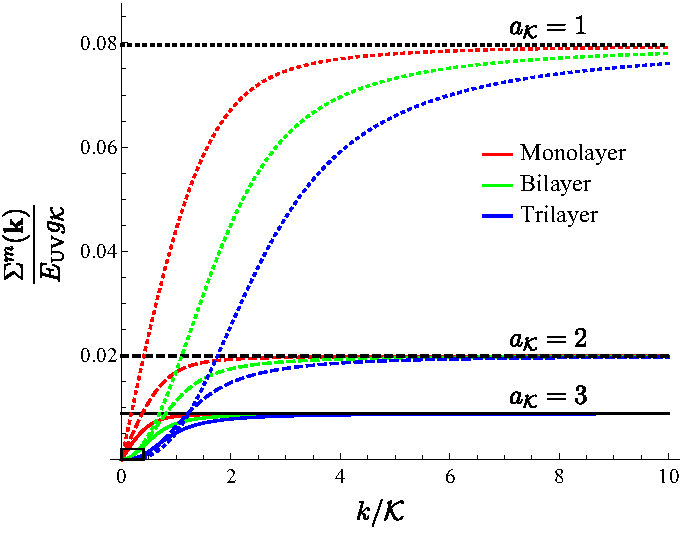
\includegraphics[scale=0.6]{SelfEnergyPlot123.pdf}
\caption{Hartree-Fock self-energy $\Sigma^{m}(\mathbf{k})$ for monolayer ($m=1$, red), bilayer ($m=2$, green) and trilayer ($m=3$, blue) graphene. The dashing of the plots represent the value of the spreading parameter: $a_{\mathcal{K}}=1$ (dotted), $a_{\mathcal{K}}$ (dashed), and $a_{\mathcal{K}}=3$ (solid), while the horizontal black lines represent the asymptotic limit $\Sigma^{m}(\infty)$ the three values of $a_{\mathcal{K}}$. The little rectangle at the origin is zoomed in Fig. \ref{fig:Multilayer-Self-Energies-Taylor}.}
\label{fig:Multilayer-Self-Energies}

\end{figure}
\begin{figure}[h]
\centering
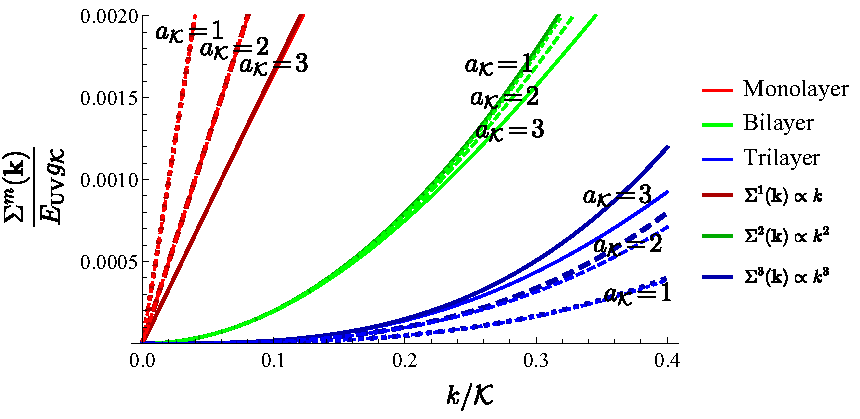
\includegraphics[scale=0.6]{SelfEnergyPlot123Taylor.pdf}
\caption{Low-momentum limit for $\Sigma^{m}(\mathbf{k})$ in monolayer, bilayer and trilayer graphene. The legends are the same shown in Fig. \ref{fig:Multilayer-Self-Energies} with the additional bolded curves representing the lowest-order expansion terms and labels of $a_{\mathcal{K}}$ to help with the interpretation of the plot. Notice that the low-momentum limit of $\Sigma^{2}(\mathbf{k})$ is independent of $a_{\mathcal{K}}$.}
\label{fig:Multilayer-Self-Energies-Taylor}
\end{figure}

\subsection{Coulombic Potential}
\label{sect:Self-Energy-Coulomb}
The Fourier potential in \eqref{eq:Fourier-Potential-Coulomb} is then replaced in \eqref{eq:General-HF-Energy}
\begin{eqnarray}
&&\Sigma^{m}(\mathbf{k })  =  \frac{E_{\mathrm{UV}}}{\mathcal{K}^{2}}
\!\!
\int \!\! \frac{d^2 \mathbf{p}}{(2\pi)^2}
\times \\
 &&\times \nonumber 
g_{\mathcal{K}} \left( 
\frac{ 
e^{-\left(\!
\tfrac{\left|\mathbf{ k-p }\right|}
{\mathcal{K}}\!\right) }
\!\!-\!
e^{-a_{\mathcal{K}} 
\left(\!
\tfrac{\left|\mathbf{ k-p }\right|}
{\mathcal{K}}\!\right) } 
}{\left|\mathbf{ k-p }\right|/\mathcal{K}}
\right) 
\cos(m\phi_{\mathbf{ k p}}),
\end{eqnarray}

The self-energy of the $m$-layer graphene is then expressed as
\begin{eqnarray}
\!\!&&\Sigma^{m}(\mathbf{k })
 = 
\frac{g_{\mathcal{K}}E_{\mathrm{UV}} k}{4 \mathcal{K}} 
\times \\ \!\! &&\times 
\left[ 
I_{\frac{m-1}{2}}\!\!
\left(\! \frac{k}{2\mathcal{K}} \!\right) \!\!
K_{\frac{m-1}{2}}\!\!
\left(\! \frac{k}{2\mathcal{K}} \!\right)
\!\! + \!
I_{\frac{m+1}{2}}\!\!
\left(\! \frac{k}{2\mathcal{K}} \!\right) \!\!
K_{\frac{m+1}{2}}\!\!
\left(\! \frac{k}{2\mathcal{K}} \!\right)
\!
\right]
\!
, \nonumber 
\end{eqnarray}
The two limit cases for large and small momenta are given by the following expressions:
\begin{equation}
\begin{split}
\lim_{k\rightarrow \infty} \Sigma^{m}(\mathbf{k }) &=
\frac{g_{\mathcal{K}}E_{\mathrm{UV}}}{2} \\
\lim_{k\rightarrow 0} \Sigma^{m}(\mathbf{k }) &=
\frac{m g_{\mathcal{K}} E_{\mathrm{UV}}}{2(m^{2}-1)}\left( \frac{k}{\mathcal{K}} \right), \quad m>1,
\end{split}
\end{equation}
It is found a similar behavior for large momenta like the Gaussian potential, but for small momenta, excepting $m=1$, the leading order is always linear in $k/\mathcal{K}$, regardless the number of layers $m$, highly in contrast to the Gaussian case where the leading order is proportional to $(k/\mathcal{K})^{m}$.
\\

	ARREGLAR EXPRESIONES Y EXPLICAR EL CASO $m=1$
\\

As special cases, the self-energy corresponding to any odd-layer and bilayer graphene are
\begin{equation}
\begin{split}
\!\!\!\!\Sigma^{n}\!(\mathbf{k })
\! &= \!
\frac{g_{\mathcal{K}}E_{\mathrm{UV}}}{8a_{\mathcal{K}}}
\frac{k e^{-\frac{a_{\mathcal{K}}^{2}k^{2}}{4\mathcal{K}^{2}}}}{\mathcal{K}\sqrt{2\pi}}
\!\!
\left[ 
\!
I_{n}\!\!
\left(\!
\frac{a_{\mathcal{K}}^{2}k^{2}}{4\mathcal{K}^{2}}
\!\right)
\!\! + \!
I_{n+1}\!\!
\left(\!
\frac{a_{\mathcal{K}}^{2}k^{2}}{4\mathcal{K}^{2}}
\!\right)
\!
\right]
\!
,
\end{split}
\end{equation}
\begin{equation}
\begin{split}
\Sigma^{2}(\mathbf{k })
\! &= \!
\frac{g_{\mathcal{K}}E_{\mathrm{UV}}}{8a_{\mathcal{K}}}
\frac{k e^{-\frac{a_{\mathcal{K}}^{2}k^{2}}{4\mathcal{K}^{2}}}}{\mathcal{K}\sqrt{2\pi}}
\!\!
\left[ 
I_{\frac{1}{2}}\!\!
\left(\!
\frac{a_{\mathcal{K}}^{2}k^{2}}{4\mathcal{K}^{2}}
\!\right)
\!\! + \!
I_{\frac{3}{2}}\!\!
\left(\!
\frac{a_{\mathcal{K}}^{2}k^{2}}{4\mathcal{K}^{2}}
\!\right)
\!
\right]
\! \\ &= \!
\frac{g_{\mathcal{K}}E_{\mathrm{UV}}}{4\pi a_{\mathcal{K}}^{2}}
\left[
1 - 
\frac{2\mathcal{K}^{2}}{a_{\mathcal{K}}^{2}k^{2}}
\left(
1-e^{-\frac{a_{\mathcal{K}}^{2}k^{2}}{2\mathcal{K}^{2}}}
\right)
\right]
\!
,
\end{split}
\end{equation}
where $n$ is an odd integer (see the Fig. \ref{fig:Multilayer-Self-Energies} for the cases of monolayer, bilayer and trilayer graphene). Their corresponding small-momentum regimes are described by
\begin{equation}
\begin{split}
\Sigma^{1}\!(\mathbf{k })
 &\approx 
\frac{g_{\mathcal{K}}E_{\mathrm{UV}}}
{8 \sqrt{2 \pi } a_{\mathcal{K}}}
\!
\left( \frac{k}{\mathcal{K}} \right)
+ O(k^{2})
, \\
\Sigma^{2}(\mathbf{k })
 &\approx 
\frac{g_{\mathcal{K}}E_{\mathrm{UV}}}
{16\pi }
\!\! 
\left( \frac{k}{\mathcal{K}} \right)^2
\!\!
+ O(k^{3})
, \\
\Sigma^{3}(\mathbf{k })
 &\approx 
\frac{a_{\mathcal{K}} E_{\mathrm{UV}}}
{64 \sqrt{2} \sqrt{\pi }}
\!\! 
\left( \frac{k}{\mathcal{K}} \right)^3
\!\!
+ O(k^{4})
,
\end{split}
\end{equation}
Notice that the dependence on $a_{\mathcal{K}}$ of the lowest-expansion-term coefficient for $\Sigma^{1}(\mathbf{k })$ is inverse to the dependence of $\Sigma^{3}(\mathbf{k })$. Even more, the lowest-expansion-term coefficient for $\Sigma^{2}(\mathbf{k })$ is independent of $a_{\mathcal{K}}$, as it is shown in Fig. \ref{fig:Multilayer-Self-Energies-Taylor}. 

\begin{figure}[h]
\centering
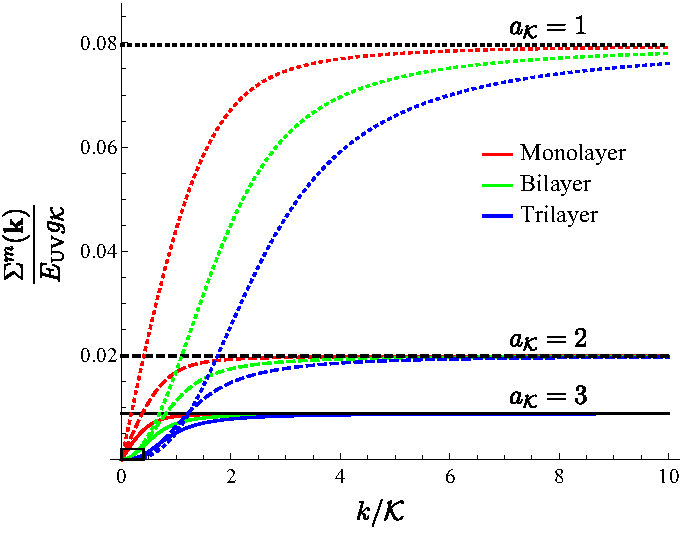
\includegraphics[scale=0.6]{SelfEnergyPlot123.pdf}
\caption{Hartree-Fock self-energy $\Sigma^{m}(\mathbf{k})$ for monolayer ($m=1$, red), bilayer ($m=2$, green) and trilayer ($m=3$, blue) graphene. The dashing of the plots represent the value of the spreading parameter: $a_{\mathcal{K}}=1$ (dotted), $a_{\mathcal{K}}$ (dashed), and $a_{\mathcal{K}}=3$ (solid), while the horizontal black lines represent the asymptotic limit $\Sigma^{m}(\infty)$ the three values of $a_{\mathcal{K}}$. The little rectangle at the origin is zoomed in Fig. \ref{fig:Multilayer-Self-Energies-Taylor}.}
\label{fig:Multilayer-Self-Energies-Coulomb}

\end{figure}
\begin{figure}[h]
\centering
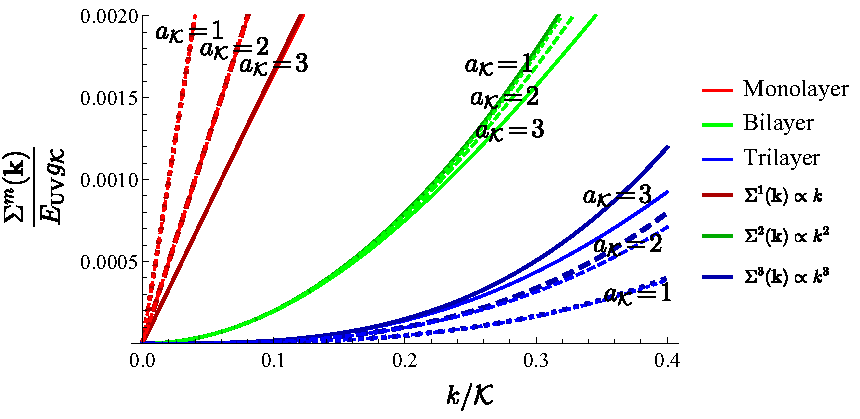
\includegraphics[scale=0.6]{SelfEnergyPlot123Taylor.pdf}
\caption{Low-momentum limit for $\Sigma^{m}(\mathbf{k})$ in monolayer, bilayer and trilayer graphene. The legends are the same shown in Fig. \ref{fig:Multilayer-Self-Energies} with the additional bolded curves representing the lowest-order expansion terms and labels of $a_{\mathcal{K}}$ to help with the interpretation of the plot. Notice that the low-momentum limit of $\Sigma^{2}(\mathbf{k})$ is independent of $a_{\mathcal{K}}$.}
\label{fig:Multilayer-Self-Energies-Taylor-Coulomb}
\end{figure}

\section{Angular momentum channels and parametrization of the radial coordinate}

\subsection{General coordinate transformations on the continuum limit}
We begin by taking the continuum limit of the Hamiltonian in the Bogoliubov basis \eqref{eq:HP-Hamiltonian}, for this purpose it is convenient to define a rescaled Hamiltonian and boson creation operator as follows: 
\begin{equation}
\begin{split}
    B(\mathbf{k}) &\equiv \lim_{\Delta k\rightarrow 0} \frac{B_{\mathbf{k}}}{\sqrt{\Delta k_{x}\Delta k_{y}}},\\
    H(\mathbf{k },\mathbf{k'}) &\equiv \lim_{\Delta k \rightarrow 0}
    \frac{H_{\mathbf{kk'}}}{\Delta k_{x}\Delta k_{y}},
\end{split}
\end{equation}
where $\Delta k_{x,y}=2\pi/\sqrt{A}$, $A$ is the system area that we take to be a square. The above re-definitions allow to obtain the following continuum commutation relations for the boson operators:
\begin{equation*}
    \left[
B(\mathbf{k }),
B^{\textcolor{black}{\dagger}}(\mathbf{k'})
\right] = \lim_{\Delta k\rightarrow 0}  \mathbb{I}\frac{\delta_{\mathbf{k k'}}}{(\Delta k)^2}
    = \mathbb{I}\delta^{2}(\mathbf{k-k'}),
\end{equation*}
where 
\begin{equation}
\mathbb{I} = 
\begin{pmatrix}
1	&	0	\\	0	&	-1	
\end{pmatrix}.
\end{equation}
With these rescalings we can convert the sums over momenta into continuum integrals, obtaining the continuum version of the boson Hamiltonian $H_{HP}$ from Eq. \eqref{eq:HP-Hamiltonian}:
\begin{equation*}
\begin{split}
\mathcal{H}_{HP} =& \lim_{\Delta k\rightarrow 0} \int \!\!
\frac{d^{2}k }{(\Delta k)^2}
\frac{d^{2}k'}{(\Delta k)^2}
B_{\mathbf{k }}^{\textcolor{black}{\dagger}}
H_{\mathbf{k } \mathbf{k'}}
B_{\mathbf{k'}}^{\textcolor{white}{\dagger}}\\
 =& \lim_{\Delta k\rightarrow 0} (\Delta k)^4 \!\! \int \!\!
\frac{d^{2}k }{(\Delta k)^2}
\frac{d^{2}k'}{(\Delta k)^2}
%\frac{
B_{\sigma }^{\textcolor{black}{\dagger}}(\mathbf{k })
%}{\Delta k}
%\frac{
H(\mathbf{k },\mathbf{k'})
%}{(\Delta k)^2}
%\frac{
B_{\sigma 
}^{\textcolor{white}{\dagger}}(\mathbf{k'})
%}{\Delta k}
\\
 =& \int \! d^{2}k d^{2}k'
%\frac{
\hat{B}_{\sigma }^{\textcolor{black}{\dagger}}(\mathbf{k })
%}{\Delta k}
%\frac{
H(\mathbf{k },\mathbf{k'})
%}{(\Delta k)^2}
%\frac{
\hat{B}_{\sigma 
}^{\textcolor{white}{\dagger}}(\mathbf{k'})
.
\end{split}
\end{equation*}

From this continuum Hamiltonian we can perfom a change of coordinates $\mathbf{k}(\mathbf{z})$ with Jacobian $D(\mathbf{z})=|\frac{\partial \mathbf{k}}{\partial \mathbf{z}}|$ with the following redefinitions:
\begin{equation}
\begin{split}
    B(\mathbf{z}) &= \sqrt{D(\mathbf{z})} 
    B(\mathbf{k}\Scale[0.9]{(\mathbf{z})}),
    \\
    H(\mathbf{z },\mathbf{z'})  &= \sqrt{D(\mathbf{z})D(\mathbf{z'})}
    H(\mathbf{k\Scale[0.9]{(\mathbf{z })}},\mathbf{k\Scale[0.9]{(\mathbf{z'})}}),
\end{split}
\end{equation}
whose purpose is to mantain the same form of the commutation relations and the Hamiltonian as follows:
\begin{equation*}
\begin{split}
&\left[
B(\mathbf{z }),B^{\textcolor{black}{\dagger}}(\mathbf{z'}) \right] =
\mathbb{I}\delta^{2}(\mathbf{z-z'}),
\\
&\mathcal{H}_{HP}
 = \int d^{2}z d^{2}z'
%\frac{
\hat{B}_{\sigma }^{\textcolor{black}{\dagger}}(\mathbf{z })
%}{\Delta k}
%\frac{
H(\mathbf{z },\mathbf{z'})
%}{(\Delta k)^2}
%\frac{
\hat{B}_{\sigma 
}^{\textcolor{white}{\dagger}}(\mathbf{z'})
.
\end{split}
\end{equation*}

Lastly, on the new coordinate system, we proceed to re-discretize the expressions, as follows:
\begin{equation}
\begin{split}
    B_{\mathbf{z}} &\leftarrow \sqrt{\Delta z_{1}\Delta z_{2}} 
    B(\mathbf{z}),
    \\
    H_{\mathbf{z },\mathbf{z'}} &\leftarrow \Delta z_{1}\Delta z_{2} \,
    H(\mathbf{z},\mathbf{z'}),
\end{split}
\end{equation}
that yield the new discrete commutation relations and Hamiltonian
\begin{equation*}
\begin{split}
\left[
B^{\textcolor{white}{\dagger}}_{\mathbf{z }},
B^{\textcolor{black}{\dagger}}_{\mathbf{z'}}
\right] &= 
\mathbb{I} \delta_{\mathbf{zz'}} 
\leftarrow \mathbb{I} 
\Delta k_{1} \Delta k_{2}  
\delta^{2}(\mathbf{z-z'})
%\\
%&= \mathbb{I} 
%\Delta k_{1} 
%\delta(z_{1}-z'_{1}) \,
%\Delta k_{2}  
%\delta(z_{2}-z'_{2})
%\\
%&= \mathbb{I}
%\delta_{z_{1}z_{1}'}
%\delta_{z_{2}z_{2}'},
\end{split}
\end{equation*}
\begin{equation}
\label{eq:Supp:Complete-Hamiltonian-Bogoliubov}
H_{HP} = \sum_{\mathbf{z},\mathbf{z'}}
B_{\mathbf{z }}^{\textcolor{black}{\dagger}}
H_{\mathbf{z }\mathbf{z'}}
B_{\mathbf{z'}}^{\textcolor{white}{\dagger}}.
\end{equation}
Therefore, in summary, the relation between operators and the Hamiltonian matrix in the new lattice defined by the discretization of the coordinates $\mathbf{z}(\mathbf{k})$, with the original operators and Hamiltonian of the square lattice is:
\begin{equation}
\label{eq:Supp:Lattice-transformations}
\begin{split}
B_{\mathbf{z}} &= \sqrt{D(\mathbf{z})\frac{\Delta z_{1}\Delta z_{2}}{\Delta k_{x}\Delta k_{y}}} 
B_{\mathbf{k}}  \\
H_{\mathbf{z }\mathbf{z'}} &= \sqrt{D(\mathbf{z })D(\mathbf{z'})}
\frac{\Delta z_{1}\Delta z_{2}}{\Delta k_{x}\Delta k_{y}}
H_{\mathbf{k }\mathbf{k'}}
\end{split}
\end{equation}
The idea is that the Hamiltonian $H_{HP}$ in Eq. \eqref{eq:Supp:Complete-Hamiltonian-Bogoliubov} will produce the same physical results as the one in the square lattice in Eq. \eqref{eq:HP-Hamiltonian} of the main text in the thermodynamic limit.

\subsection{Polar re-discretization}

We choose $\mathbf{z}=(k,\phi)$ where $k$ is the radius of the momentum vector and $\phi$ its polar angle. We then discretize the radial direction in two different ways specified below to check numerically that the precise form of the discretization is not crucial to the results. Therefore we choose the radial coordinate as:
\begin{equation}
\label{eq:Supp:Tangential-radius}
\begin{split}
    k &= k(\theta) \rightarrow k_{n} = k(\theta_{n},\Delta \theta), 
\end{split}
\end{equation}
where $\theta$ is another parameter labeling the radial coordinate that we will choose to be uniformly discretized. The corresponding Jacobian for this parametrization is:
\begin{equation}
\label{eq:Supp:Jacobian}
\begin{split}
    D(\theta) &= k(\theta)\frac{dk(\theta)}{d\theta}.
\end{split}
\end{equation}

\begin{figure}[b]
\centering
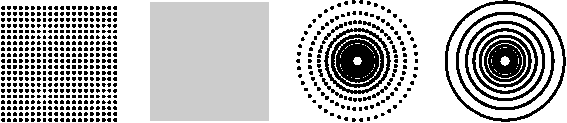
\includegraphics[scale=0.8]{SquarePolarLattice.pdf}
\caption{Depiction of the re-discretization procedure, from the initial square through the continuum limit of the system to the polar lattice and the integration of the angular coordinate in angular momentum channels reducing the dimensionality of the system to 1.}
\end{figure}

The parameters $\theta$ and $\phi$ are uniformly discretized as follows:
\begin{equation}
\label{eq:Supp:Discretization-of-angles}
\begin{split}
\theta_{n} &= n \Delta\theta, \quad m \in \{1,\cdots ,N\}, \\
  \phi_{l} &= l \Delta\phi  , \quad \:n \,\in \{-L,\cdots ,L\},
\end{split}
\end{equation}
where $N$ is the total number of slices of the radial coordinate and $2L+1$ is the total number of slices for the angular coordinate, and
\begin{equation}
\label{eq:Discrete-angle-units}
\Delta \theta = \Delta \theta(N), 
\quad
\Delta \phi = \frac{2\pi}{2L + 1}.
\end{equation}
The actual form of $k(\theta_{n},\Delta \theta)$ is determined by the particular discretization used to calculate the matrix elements of the Hamiltonian (more details in \S \ref{sect:description-num-proc}).
Therefore, the new polar lattice is determined by the sites $\mathbf{z}=(k_{n},\phi_{l})$ where:
\begin{equation}
\label{eq:Tangential-radius}
\begin{split}
    k_{n} &= k(n,\Delta \theta),
    \quad \phi_{l} = l\Delta \phi,
\end{split}
\end{equation}


After replacing \eqref{eq:Supp:Tangential-radius} and  \eqref{eq:Supp:Jacobian} into \eqref{eq:Supp:Lattice-transformations} we get the expression for $B_{\mathbf{k}}$ and $H_{\mathbf{k k'}}$ in the polar lattice
\begin{equation}
\label{eq:Supp:Lattice-transformations-1}
\begin{split}
B_{n}^{l\textcolor{white}{\dagger}} &=
\frac{\mathcal{K}\sqrt{A}}{2\pi}
\sqrt{\Delta \theta \Delta \phi D_{n} }
B_{\mathbf{k}_{nl}}^{\textcolor{black}{\dagger}},  \\
H_{nn'}^{ll'} &= 
\frac{\mathcal{K}^{2}A}{(2\pi)^{2}}
\Delta \theta \Delta \phi 
\sqrt{D_{n}D_{n'}}
H_{\mathbf{k}_{nl}\mathbf{k}_{n'l'}},
\end{split}
\end{equation}
where $D_{n}=D(n\Delta \theta)$ and $\mathbf{k}_{nl}=\mathbf{k}(\theta_{n},\phi_{l})$. Finally, the whole Hamiltonian is
\begin{equation}
H_{HP} = \sum_{nl}\sum_{n'l'}
B_{n }^{l \textcolor{black}{\dagger}}
H_{nn'}^{ll'}
B_{n'}^{l'\textcolor{white}{\dagger}}.
\end{equation}

\subsection{Angular momentum channels}
Because the Hamiltonian matrix $H_{\mathbf{k k'}}$ that enters into the Hamiltonina $H_{HP}$ in Eq. \eqref{eq:HP-Hamiltonian} of the main text only depends on the difference between the polar angles $\phi-\phi'$ we have conservation of the angular momentum $l$ of the bosons. Consequently, we perform Fourier transforms on the polar angles for the fields $B_{mn}$ and the matrix $H_{mn,m'n'}$
\begin{equation}
\begin{split}
B_{n}^{l\textcolor{white}{\dagger}} &= 
\frac{1}{\sqrt{2L+1}}\sum_{\ell=-L}^{L}
e^{-i \ell \phi_{l}}B_{n}^{\ell} ,
\\
H_{nn'}^{ll'} &= \sum_{\ell=-L}^{L}
e^{-i \ell (\phi_{l }-\phi_{l'})}
H_{mm'}^{\ell},
\end{split}
\end{equation}
such that the total Bogoliubov Hamiltonian decomposes into a direct sum for different angular mommentum channels, as follows:
\begin{equation}
H_{HP} = \sum_{nn'\ell}
B_{n  }^{\ell\textcolor{black}{\dagger}}
H_{nn'}^{\ell}
B_{n' }^{\ell}.
\end{equation}

In that way, each dataset obtained from diagonalizing a $2N\times 2N$ matrix is labelled by the coupling constant $g_{\mathcal{K}}$ and spreading $a_{\mathcal{K}}$ of the Gaussian potential, the number of layers $m=2$ fixed for bilayer graphene, the angular momentum $\ell$ and the number of sites in the radial coordinate $N$.



\section{Numerical results}

\subsection{Description of the numerical procedure}
\label{sect:description-num-proc}

The solution of the system is found with exact diagonalization of the $2N\times 2N$ matrix composed by the matrix elements of the Hamiltonian for the hopping ($b^{\textcolor{black}{\dagger}}_{k_{1}}\!b^{\textcolor{white}{\dagger}}_{k_{2}}$) and pairing ($b^{\textcolor{white}{\dagger}}_{k_{1}}\!b^{\textcolor{white}{\dagger}}_{k_{2}},$ $b^{\textcolor{black}{\dagger}}_{k_{1}}\!b^{\textcolor{black}{\dagger}}_{k_{2}}$) terms. The parameters of the Hamiltonian are:
\begin{itemize}
\item Angular momentum $\ell=$ 0, 1, 2, 3, 4, 5.
\item Coupling constant $a_{\mathcal{K}}=$ 1, 2, 5, 10.
\item Reciprocal spreading $a_{\mathcal{K}}=$ 1, 2, 5, 10.
\item System size $N=$ 100, 200, 300, 400, 500.
\end{itemize}
and the UV-cutoff being set to the unity, i.e., $\mathcal{K}=1$ and $E_{\mathrm{UV}}=1$.

Regarding the spacing of the lattice for the radial component of the momentum $k_{n}=k(\theta_{n},\Delta \theta)$, the following four parametrizations were taken into account to show that at the infinite size limit $N\rightarrow \infty$ the results do not depend on the discretization: 
\begin{itemize}
\item Discretization by powers of $n$ ($R=1,2$):
\begin{equation}
\label{eq:Discretization-powers}
k_{n} = \mathcal{K}\left( n \Delta \theta \right)^{R},
\end{equation}
with Jacobian given by
\begin{equation}
D_{n} = \mathcal{K}^{2}R 
\Delta k\left(n\Delta \theta\right)^{2R-1},
\end{equation}
and spacing
\begin{equation}
\Delta \theta = 1/N.
\end{equation}
\item Discretization by tangent of $n$ ($R=1,2$):
\begin{equation}
\label{eq:Discretization-tangents}
k_{n} = \frac{\mathcal{K}}{\sqrt{R}}\tan^{R}
\left(n\Delta \theta\right)
\end{equation}
with Jacobian given by
\begin{equation}
D_{n} = \mathcal{K}^{2} \Delta \theta 
\sec^{2}\left(n\Delta \theta\right)
\tan^{2R-1} \left(n\Delta \theta\right),
\end{equation}
and spacing
\begin{equation}
\Delta \theta = \frac{\pi/2}{N+1}
\end{equation}
\end{itemize}
Consequently, the Hamiltonians spanned by the parameter space $\{\ell,g_{\mathcal{K}},a_{\mathcal{K}},N,R\}$ are obtained using the parametrizations of the radial coordinate $k_{n}$, then the infinite size limit $N\rightarrow \infty$ is taken to ensure that the results are independent of the particular discretization chosen during the numerical procedures.

\subsection{Imaginary eigenvalues after doing exact diagonalization}

\begin{figure*}
\centering 
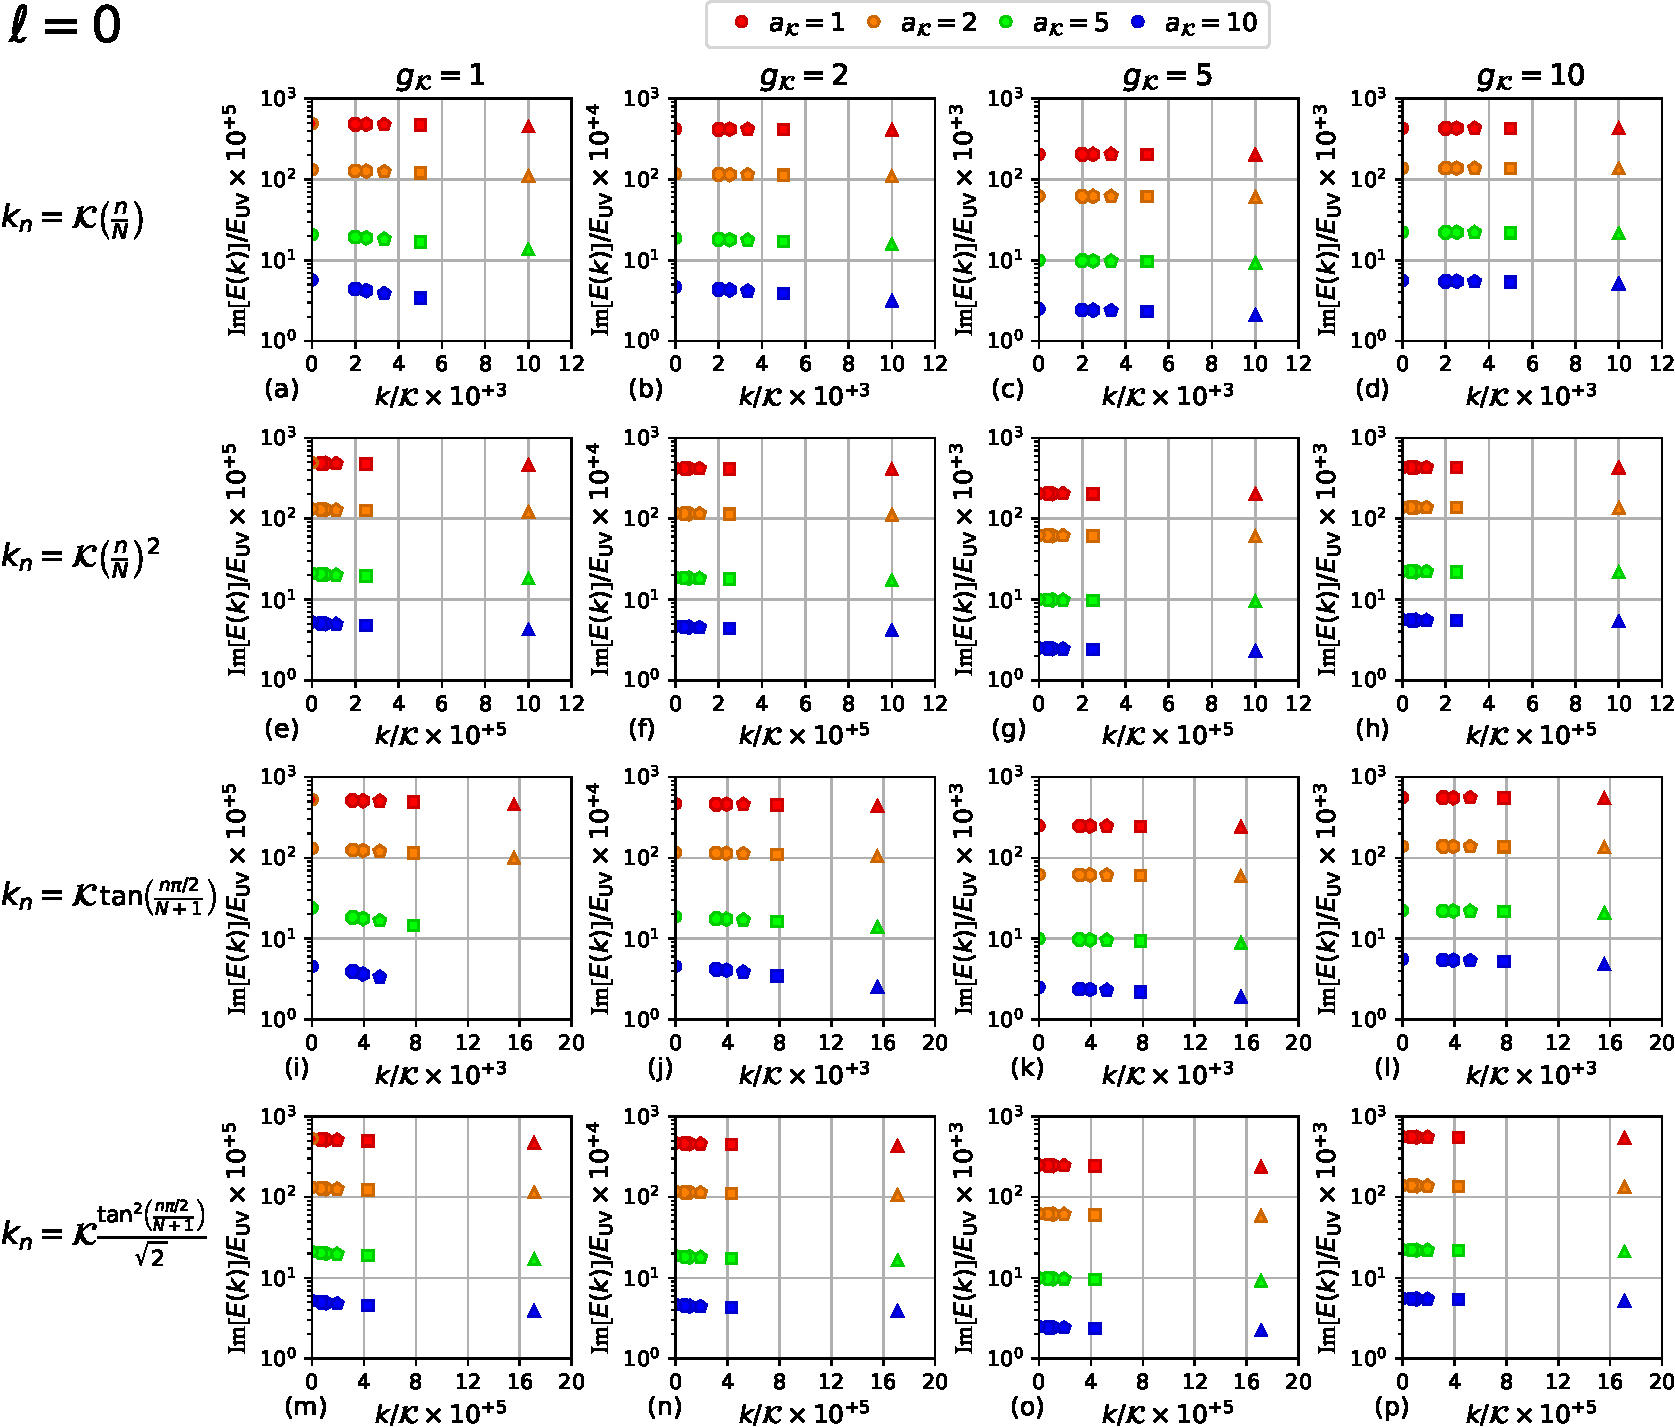
\includegraphics[scale=0.5]{./PlotReport/PlotReportL0.pdf}
\caption{Imaginary parts of the eigenvalues corresponding to the smallest momentum $k_{1}$ for $\ell=0$ and different system sizes $N$: $\triangle$ ($N=100$), $\square$ ($N=200$), $\largepentagon$ ($N=300$), $\largevarhexagon$ ($N=400$), and $\octagon$ ($N=500$). The extrapolation is $\ocircle$ for $N\rightarrow \infty$. }
\label{fig:PlotReportL0}
\end{figure*}

\begin{figure*}
\centering 
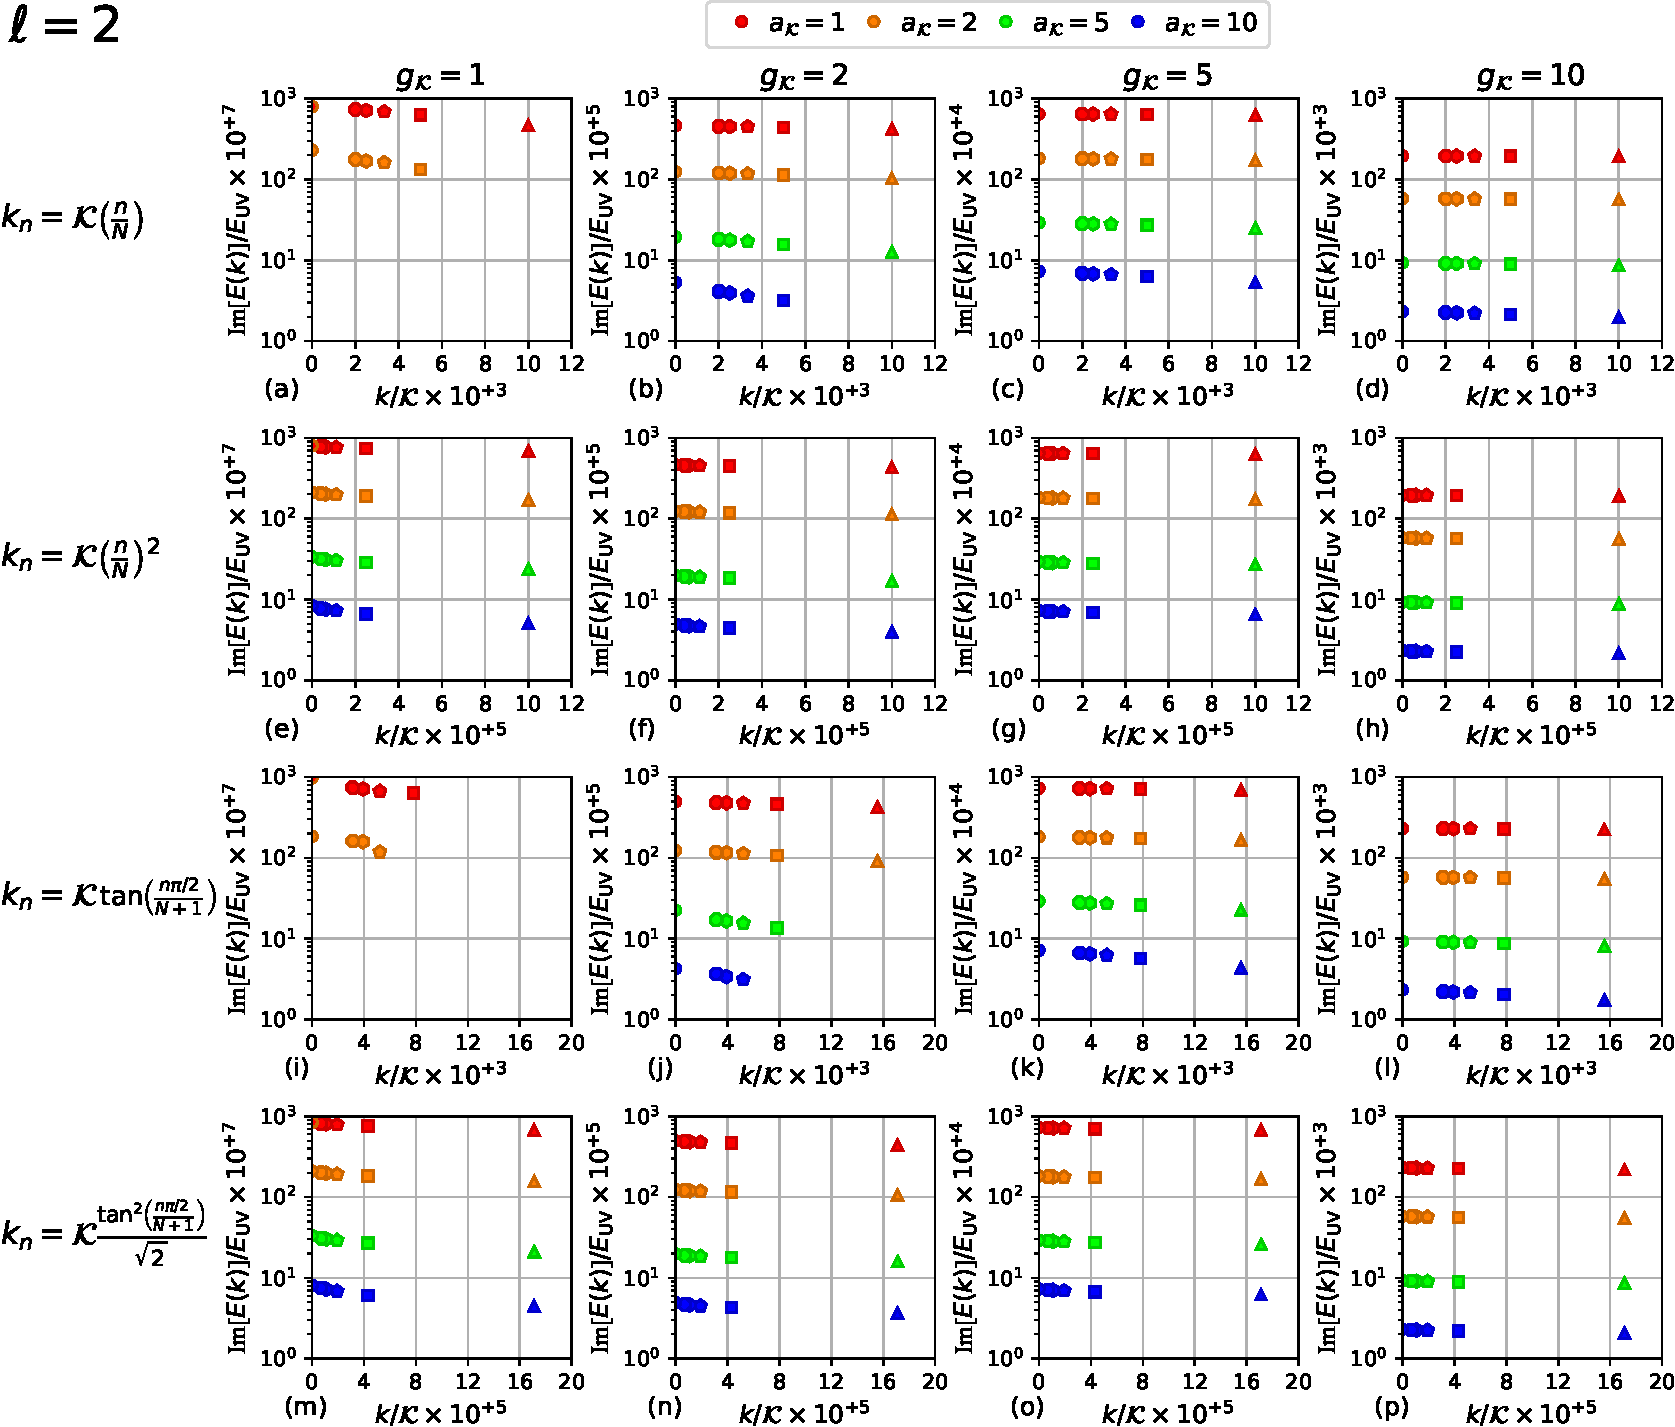
\includegraphics[scale=0.5]{./PlotReport/PlotReportL2.pdf}
\caption{Imaginary parts of the eigenvalues corresponding to the smallest momentum $k_{1}$ for $\ell=2$ and different system sizes $N$: $\triangle$ ($N=100$), $\square$ ($N=200$), $\largepentagon$ ($N=300$), $\largevarhexagon$ ($N=400$), and $\octagon$ ($N=500$). The extrapolation is $\ocircle$ for $N\rightarrow \infty$. }
\label{fig:PlotReportL2}
\end{figure*}

The Hamiltonian was diagonalized for the different sets of the parameter space $\{\ell, g_{\mathcal{K}}, a_{\mathcal{K}},N,R\}$, and then the energy spectra were examined looking for non-vanishing imaginary parts $\mathrm{Im}[E(k)]$ pointing out to an unstability in the modes of the system. The only two angular momentum channels that got non-vanishing imaginary parts in their eigenvalue spectra were $\ell=0$ and $\ell=2$, both showing only one eigenvalue with imaginary part (with the corresponding complementary eigenvalue with the opposite sign) at the site $n=1$, corresponding to the smallest momentum, 
\begin{equation}
\mathrm{Im}[E(k_{\mathrm{min}})] = \mathrm{Im}\left[E\left(\Delta \theta \right)\right] \neq 0,
\end{equation}
shown in the Figs. \ref{fig:PlotReportL0} and \ref{fig:PlotReportL2} for $\ell=0$ and $\ell=2$, respectively. Since the imaginary eigenvalues show a finite asympthotic trend when $k_{\mathrm{min}}\rightarrow 0$, i.e., $N\rightarrow\infty$, the five values obtained for each system size are taken to get the infinite size limit shown as the circles $\ocircle$ in the forementioned figures. 
\\

As expected, although the four discretizations of $k_{n}$ yield different numerical results depending on the power $R$, the form of $k(n,\Delta k)$ (powers in Eq. \eqref{eq:Discretization-powers} or tangents in Eq. \eqref{eq:Discretization-tangents}), or the system size $N$, the infinite system size limit $N\rightarrow \infty$ where $k_{1}\rightarrow 0$ yields almost the same imaginary eigenvalues, with a slight increment for the tangent discretization produced by the contribution of the sites along the radial momentum beyond the UV-cutoff $\mathcal{K}$, in other words, the sites $k_{n}$ with $n>N/2$.

There are some plots for small $g_{\mathcal{K}}$ with $R=1$ like Fig. \ref{fig:PlotReportL0}(a) or \ref{fig:PlotReportL0}(c), or even worse in Fig. \ref{fig:PlotReportL2}(a) and \ref{fig:PlotReportL2}(c) where there are missing markers for large $a_{\mathcal{K}}$ that are shown in their analogues with $R=2$, Figs. \ref{fig:PlotReportL0}(b), \ref{fig:PlotReportL0}(d), \ref{fig:PlotReportL2}(b) and \ref{fig:PlotReportL2}(d), respectively, This fact suggests that finer lattices are required to catch the non-vanishing imaginary part of the eigenvalue corresponding to the site with the smallest momentum, $k_{1}$, supporting the fact that the imaginary eigenvalue, i.e., the instalibity, is located at momentum $k\rightarrow 0$.

The main differences between $\ell=0$ and $\ell=2$ channels root on the relative size of their imaginary eigenvalues, being smaller for the latter channel, almost a half of those ones for the former channel. On the other hand, the channels show expected behaviors like the increasing of $\mathrm{Im}[E(k_{\mathrm{min}})]$ for larger $g_{\mathcal{K}}$, i.e., stronger interactions, and the suppression for larger $a_{\mathcal{K}}$, that is, a wider spreading of the potential, turning out in a weaker interaction and consequently, smaller values for $\mathrm{Im}[E(k_{\mathrm{min}})]$.

\begin{figure}
\centering
%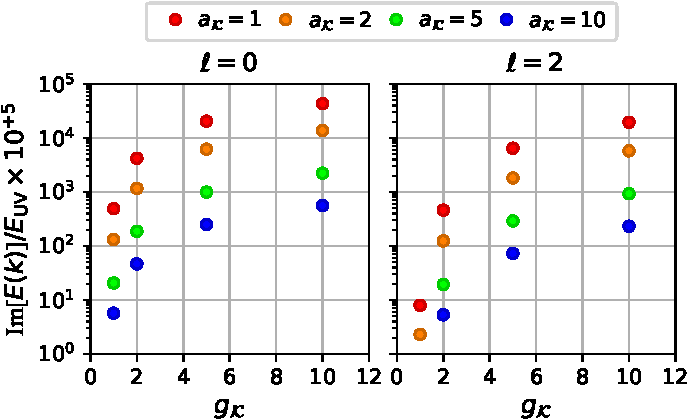
\includegraphics[scale=0.6]{./PlotReport/PlotReportPow}PlotReportPowR1L0
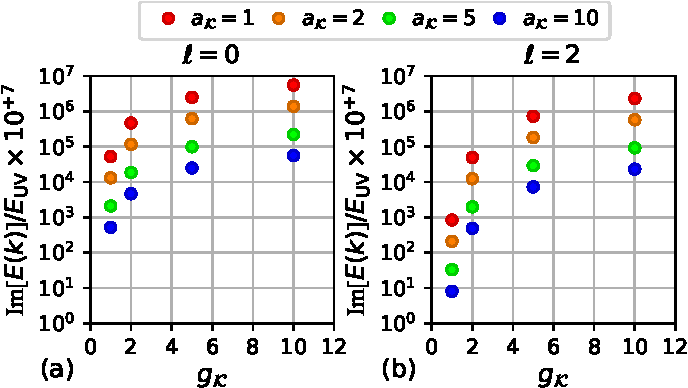
\includegraphics[scale=0.55]{./PlotReport/PlotReportTotal}
\caption{Summarize of the infinite size limit $N\rightarrow\infty$ of the imaginary parts shown in Figs. \ref{fig:PlotReportL0} and \ref{fig:PlotReportL2} vs. the coupling constant $g_{\mathcal{K}}$.}
\label{fig:PlotReport}
\end{figure}

The infinite size limits for $\mathrm{Im}[E(k_{\mathrm{min}}\rightarrow 0)]$, from now on denoted as $\mathrm{Im}[E^{\ell}](a_{\mathcal{K}},g_{\mathcal{K}})$, are obtained using the dataset found with the tangent discretization in Eq. \eqref{eq:Discretization-tangents} with $R=3$ and least-squares on the Ansatz 
\begin{equation}
\label{eq:Zero-Ansatz}
\begin{split}
\mathrm{Im}[E^{\ell}]&(a_{\mathcal{K}},g_{\mathcal{K}},N) = \\ 
&\mathrm{Im}[E^{\ell}](a_{\mathcal{K}},g_{\mathcal{K}}) + \frac{\Delta\mathrm{Im}[E^{\ell}](a_{\mathcal{K}},g_{\mathcal{K}})}{N}.
\end{split}
\end{equation}
The results are listed in the tables \ref{tab:Inf-size-points-L0} and \ref{tab:Inf-size-points-L2} for the channels $\ell=0$ and $\ell=2$, respectively, and are summarized in the Fig. \ref{fig:PlotReport} for large coupling $g_{\mathcal{K}}\geq 1$.

\subsection{Ansatz}
\begin{table*}
\centering 
\begin{tabular}{cccccccc}
&&
\multicolumn{2}{c}{$\ell=0$} &&
\multicolumn{2}{c}{$\ell=2$}\\	\hline	\hline 
$a_{\mathcal{K}}$	&&	
$C_{0}$	&	$G_{0}$ &&&
$C_{2}$	&	$G_{2}$	\\	\hline	\hline 
1	&&	
$(2.805\pm 0.020)\times 10^{-1}$	&
$ 4.020\pm 0.003$ &&&
$(2.619\pm 0.004)\times 10^{-1}$	&
$ 8.042\pm 0.001$\\
2	&&	
$(7.116\pm 0.062)\times 10^{-2}$	&
$ 4.028\pm 0.004$ &&&
$(6.697\pm 0.073)\times 10^{-2}$	&
$ 8.063\pm 0.008$\\
3	&&	
$(3.158\pm 0.014)\times 10^{-2}$	&
$ 4.027\pm 0.002$ &&&
$(2.967\pm 0.019)\times 10^{-2}$	&
$ 8.062\pm 0.005$\\
5	&&	
$(1.113\pm 0.013)\times 10^{-2}$	&
$ 4.024\pm 0.004$ &&&
$(1.078\pm 0.008)\times 10^{-2}$	&
$ 8.073\pm 0.005$\\
7	&&	
$(5.862\pm 0.058)\times 10^{-3}$	&
$ 4.035\pm 0.004$ &&&
$(5.548\pm 0.101)\times 10^{-3}$	&
$ 8.082\pm 0.014$\\
10	&&	
$(2.917\pm 0.040)\times 10^{-3}$	&
$ 4.044\pm 0.006$ &&&
$(2.783\pm 0.056)\times 10^{-3}$	&
$ 8.106\pm 0.002$
\end{tabular}
\caption{Fitting of parameters $C_{0}$ and $G_{0}$ depending on $a_{\mathcal{K}}$ to the first Ansatz in Eq. \eqref{eq:First-Ansatz}. }
\label{tab:First-Ansatz}
\end{table*}

The first Ansatz proposed by Inti consisted in the following function: 
\begin{equation}
\label{eq:First-Ansatz}
\mathrm{Im}[E^{\ell}](a_{\mathcal{K}},g_{\mathcal{K}}) = C_{\ell}(a_{\mathcal{K}})
e^{-G_{\ell}(a_{\mathcal{K}})/g_{\mathcal{K}}},
\end{equation}
where $G_{\ell}(a_{\mathcal{K}})$ and $C_{\ell}(a_{\mathcal{K}})$ are parameters to be found for each set of points labelled with $a_{\mathcal{K}}$. The points used for the fitting are the infinite-size limits $\mathrm{Im}[E^{\ell}](a_{\mathcal{K}},g_{\mathcal{K}})$ listed in the tables \ref{tab:Inf-size-points-L0} and \ref{tab:Inf-size-points-L2}. The table \ref{tab:First-Ansatz} shows the results of the fitting of the Eq. \eqref{eq:First-Ansatz} using non-linear least-squares (NLLS), and are summarized in the Fig. \ref{fig:First-Ansatz}. 

\begin{figure}
\centering
%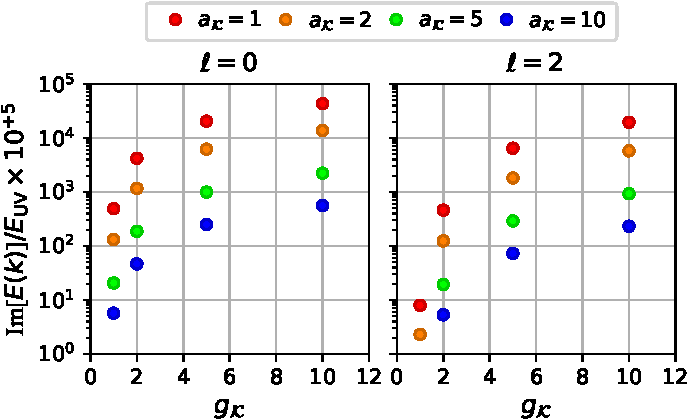
\includegraphics[scale=0.6]{./PlotReport/PlotReportPow}PlotReportPowR1L0
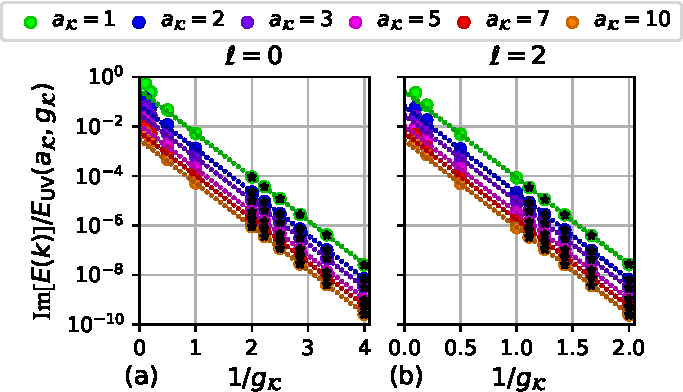
\includegraphics[scale=0.6]{./PlotReport/FirstAnsatz}
\caption{Infinite-size limits $\mathrm{Im}[E^{\ell}](a_{\mathcal{K}},g_{\mathcal{K}})$ vs. $1/g_{\mathcal{K}}$ compared to the fitted Ansatz shown in Eq. \eqref{eq:First-Ansatz}. The points used in the interpolation are highlighed with black stars. Notice the discrepancy at strong coupling $g_{\mathcal{K}}\geq 1$.}
\label{fig:First-Ansatz}
\end{figure}

In order to improve the first Ansatz, the two parameters $G_{\ell}(a_{\mathcal{K}})$ and $C_{\ell}(a_{\mathcal{K}})$ were fitted by a second NLLS procedure on two Ans\"{a}tze. The first one for $G_{\ell}(a_{\mathcal{K}})$ given by
\begin{equation}
G_{\ell}(a_{\mathcal{K}}) = G_{\ell} + a_{\mathcal{K}}\Delta G_{\ell}
\end{equation}
yielding the parameters
\begin{equation}
\label{tab:Second-Ansatz-G0-L0}
\begin{split}
G_{0}  &= 4.020\pm 0.002,	\\
\Delta G_{0} &= (2.110\pm 0.645)\times 10^{-3},
\end{split}
\end{equation}
in the channel $\ell=0$, and 
\begin{equation}
\label{tab:Second-Ansatz-G0-L2}
\begin{split}
G_{2}  &= 8.034\pm 0.002,	\\
\Delta G_{2} &= (7.782\pm 0.839)\times 10^{-3},
\end{split}
\end{equation}
in the channel $\ell=2$. Since the slope of the fittings $\Delta G_{\ell}$ are three orders of magnitude smaller than the intercept and $a_{\mathcal{K}}\sim 1$, we can assume that $G_{\ell}$ is constant respect to $a_{\mathcal{K}}$ (see Fig. \ref{fig:Second-Ansatz}(b)). Meanwhile the Ansatz for $C_{\ell}(a_{\mathcal{K}})$ is a power law 
\begin{equation}
\label{eq:Second-Ansatz}
C_{\ell}(a_{\mathcal{K}})= \left(\frac{A_{\ell}}{a_{\mathcal{K}}} \right)^{\alpha_{\ell}},
\end{equation}
whose parameters found are 
\begin{equation}
\label{tab:Second-Ansatz-L0}
\begin{split}
A_{0}  &= (5.282\pm 0.029)\times 10^{-1},	\\
\alpha_{0} &=  1.990\pm 0.006,
\end{split}
\end{equation}
in the channel $\ell=0$, and 
\begin{equation}
\label{tab:Second-Ansatz-L2}
\begin{split}
A_{2}  &= (5.084\pm 0.005)\times 10^{-1},	\\
\alpha_{2} &= 1.981\pm 0.002,
\end{split}
\end{equation}
in the channel $\ell=2$. The small errors of the parameters after the fitting suggest us that the power-law is a good Ansatz to describe $C_{\ell}(a_{\mathcal{K}})$ (see Fig. \ref{fig:Second-Ansatz}(a)).

\begin{figure}
\centering
%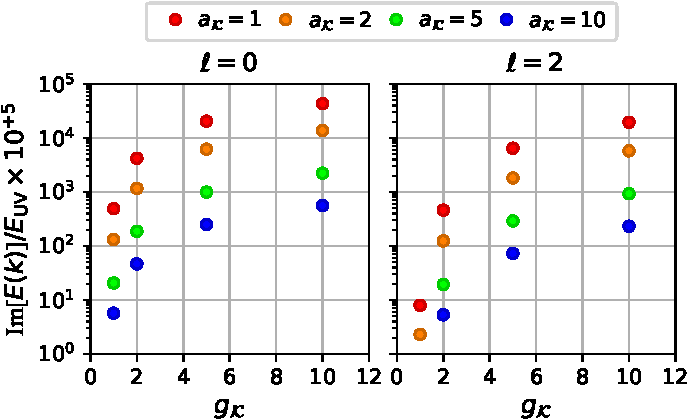
\includegraphics[scale=0.6]{./PlotReport/PlotReportPow}PlotReportPowR1L0
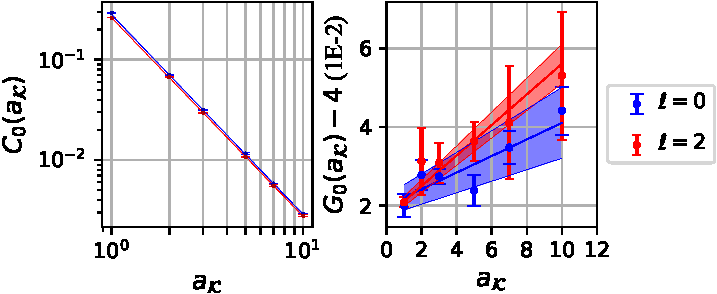
\includegraphics[scale=0.70]{./PlotReport/PlotC0G0.pdf}
\caption{Data points shown in the Tab. \ref{tab:First-Ansatz} and fitted Ans\"{a}tze. Left: $C_{0}$ vs. $a_{\mathcal{K}}$: the power law in Eq. \eqref{eq:Second-Ansatz} was fitted with the parameters in Eqs. \eqref{tab:Second-Ansatz-L0} and \eqref{tab:Second-Ansatz-L2} for $\ell=0$ and $\ell=2$. Right: $G_{0}$ vs. $a_{\mathcal{K}}$: the linear regression yielded the parameters in Eq. \eqref{tab:Second-Ansatz-G0-L0} and \eqref{tab:Second-Ansatz-G0-L2} (the data for $\ell=2$ was divided by 2 to easen the interpretation of the plot). Both figures include the error bars as well as the regions allowed by the standard errors of the fittings.}
\label{fig:Second-Ansatz}
\end{figure}

\begin{figure*}
\centering
%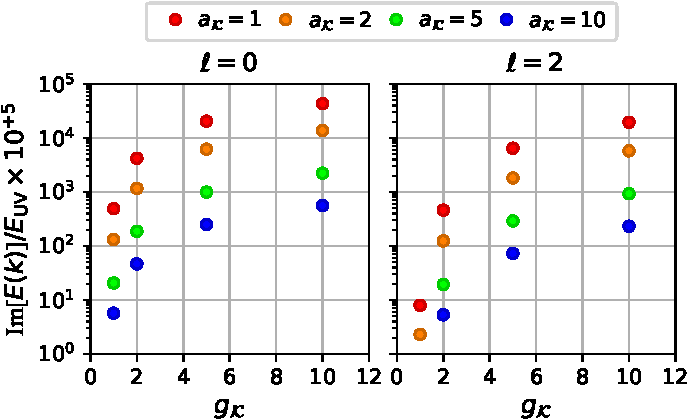
\includegraphics[scale=0.6]{./PlotReport/PlotReportPow}PlotReportPowR1L0
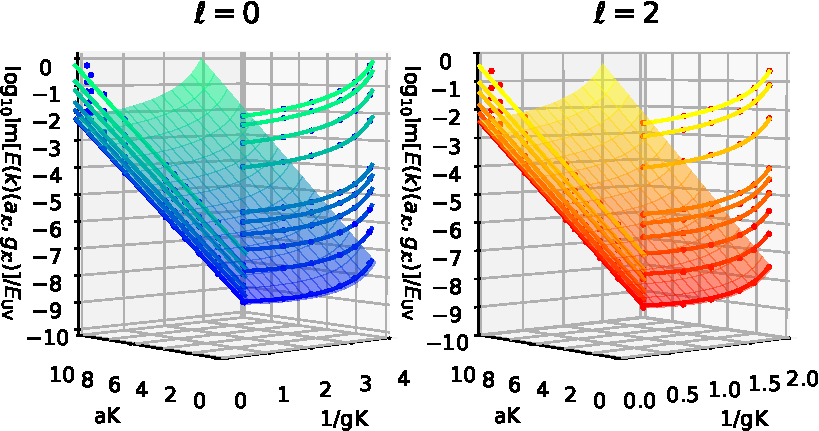
\includegraphics[scale=0.8]{./PlotReport/ThirdAnsatz.pdf}
\caption{Infinite-size limits $\mathrm{Im}[E^{\ell}](a_{\mathcal{K}},g_{\mathcal{K}})$ vs. the inverse of the coupling constant $1/g_{\mathcal{K}}$ with the fitted Ansatz shown in Eq. \eqref{eq:First-Ansatz}. The points used in the interpolation are highlighed with black stars. Notice the discrepancy at strong coupling $g_{\mathcal{K}}\geq 1$.}
\label{fig:Third-Ansatz}
\end{figure*}

Therefore, Inti's Ansatz was modified to include the new power law with $\alpha=2$ as follows:
\begin{equation}
\label{eq:Third-Ansatz}
\mathrm{Im}[E^{\ell}](a_{\mathcal{K}},g_{\mathcal{K}}) = 
\left(\frac{A_{\ell}}{a_{\mathcal{K}}} \right)^{2}
e^{-G_{\ell}/g_{\mathcal{K}}},
\end{equation}
and then fitted using two-dimensional NLLS on the plane $(a_{\mathcal{K}}, g_{\mathcal{K}})$ yielding that
\begin{equation}
\begin{split}
A_{0} &= (5.306\pm 0.015)\times 10^{-1},	\\
G_{0} &= 4.024\pm 0.002,
\end{split}
\end{equation}
in the channel $\ell=0$, and 
\begin{equation}
\begin{split}
A_{2} &= (5.135\pm 0.018)\times 10^{-1},	\\
G_{2} &= 8.050\pm 0.005,
\end{split}
\end{equation}
in the channel $\ell=2$. The fitted data as well as the Ansatz of Eq. \eqref{eq:Third-Ansatz} are shown in the Fig. \ref{fig:Third-Ansatz} including projections onto the planes $\mathrm{Im}[E^{\ell}](a_{\mathcal{K}},g_{\mathcal{K}})$  vs. $1/g_{\mathcal{K}}$ and $\mathrm{Im}[E^{\ell}](a_{\mathcal{K}},g_{\mathcal{K}})$ vs. $a_{\mathcal{K}}$. 

Lastly, the fitting also suggests a relation in te $G_{\ell}$ parameters, corresponding to the power of the exponential in Eq. \eqref{eq:Third-Ansatz}, that $G_{2}=2G_{0}$, which is consistent to the standard errors reported above. A similar conclusion may not be done on $A_{\ell}$ since the standard errors as well as the central values do not allow such overlapping. 





\section{Inti's general scheme}
The system without interactions is described by the following 2D Hamiltonian
\begin{equation}
\begin{split}
H_{\mathrm{kin}} &= \!
\int \! d^{2}r 
\Psi_{\mathbf{r}}^{\textcolor{black}{\dagger}}
\left( 
\boldsymbol{\sigma}\cdot \frac{\boldsymbol{\nabla}}{i}
\right)
\Psi_{\mathbf{r}}^{\textcolor{white}{\dagger}}
=
\sum_{\mathbf{k}} 
\Psi_{\mathbf{k}}^{\textcolor{black}{\dagger}}
\left(
\boldsymbol{\sigma}\cdot \mathbf{k}
\right)
\Psi_{\mathbf{k}}^{\textcolor{white}{\dagger}}
\end{split}
\end{equation}
where $\Psi_{\mathbf{k}}$ is the annihilation operator of the fundamental representation of $\mathrm{SU(2)}$
\begin{equation}
\Psi_{\mathbf{k}} = 
\begin{pmatrix}
\psi_{\mathbf{k}\uparrow } \\
\psi_{\mathbf{k}\downarrow }
\end{pmatrix},
\end{equation}
and the occupied state is given by the action of the creation operator on the ground state
\begin{equation}
\left| 
\mathbf{k}\sigma 
\right\rangle = 
\psi_{\mathbf{k}\sigma}^{\textcolor{black}{\dagger}}
\left| 0 \right\rangle
\end{equation}
whose time evolution is determined by the Hamiltonian
\begin{equation}
i\frac{\partial}{\partial t}
\left| 
\mathbf{k}\sigma 
\right\rangle = 
H \left| 
\mathbf{k}\sigma 
\right\rangle 
\end{equation}
The Lagrangian associated to the Hamiltonian is given by
\begin{equation}
L = i
\left\langle 
\mathbf{k}\sigma \!\!
^{\textcolor{white}{\dagger}}_{\textcolor{white}{\dagger}}
\right|
\frac{\partial}{\partial t} 
\left| 
^{\textcolor{white}{\dagger}}_{\textcolor{white}{\dagger}}\!\!
\mathbf{k}\sigma 
\right\rangle -
\left\langle 
\mathbf{k}\sigma \!\!
^{\textcolor{white}{\dagger}}_{\textcolor{white}{\dagger}}
\right|
H
\left| 
^{\textcolor{white}{\dagger}}_{\textcolor{white}{\dagger}}\!\!
\mathbf{k}\sigma 
\right\rangle 
\end{equation}

The following operator rotates the spins at every given momentum $\mathbf{k}$ around the axis $\hat{\boldsymbol{\Omega}}$ by an angle $|\boldsymbol{\Omega}|$:
\begin{equation}
\begin{split}
U(\boldsymbol{\Omega}(\mathbf{k})) &= 
\exp \left[
\frac{i}{2} \sum_{\mathbf{k}}
\boldsymbol{\Omega}(\mathbf{k}) \cdot 
\mathbf{S}_{\mathbf{k}}
\right] \\ &= 
\exp \left[
\frac{i}{2} \sum_{\mathbf{k}}
\boldsymbol{\Omega}(\mathbf{k}) \cdot 
\left(
\Psi_{\mathbf{k}}^{\textcolor{black}{\dagger}}
\boldsymbol{\sigma}
\Psi_{\mathbf{k}}^{\textcolor{white}{\dagger}}
\right)
\right]
\end{split}
\end{equation}
where $\mathbf{S}_{\mathbf{k}} = \Psi_{\mathbf{k}}^{\textcolor{black}{\dagger}}
\boldsymbol{\sigma}
\Psi_{\mathbf{k}}^{\textcolor{white}{\dagger}}$ is the spin operator. 
Consider the case of a single spin $\sfrac{1}{2}$
\begin{equation}
\begin{split}
U(\boldsymbol{\Omega}(\mathbf{k})) &= 
\exp \left[
\frac{i}{2} 
\boldsymbol{\Omega} \cdot 
\left(
\Psi^{\textcolor{black}{\dagger}}
\boldsymbol{\sigma}
\Psi%^{\textcolor{white}{\dagger}}
\right)
\right]
\end{split}
\end{equation}
The action of $U(\boldsymbol{\Omega})$ on $\sigma_{i}$ is obtained using the well-known Backer-Campbell-Haussdorf formula (BCH):
\begin{equation}
\begin{split}
&U^{\dagger}(\boldsymbol{\Omega})
\sigma_{i}
U(\boldsymbol{\Omega}) \approx \\ &\approx 
\sigma_{i} - \frac{i}{2}\Omega^{j}
\left[ \sigma_{j},\sigma_{i} \right]
+ \left(\frac{-i}{2}\right)^{2}
\frac{\Omega^{j}\Omega^{k}}{2!}
\left[ \sigma_{j},\left[ \sigma_{k},\sigma_{i} \right] \right] \\ &= 
\sigma_{i} - \frac{i}{2}\Omega^{j}
2i\epsilon_{ji}^{\;\;\,k}\sigma_{k}
+ \left(\frac{-i}{2}\right)^{2}
\frac{\Omega^{j}\Omega^{k}}{2!}
\left[ \sigma_{j},2i\epsilon_{ki}^{\;\;\;l}\sigma_{l} \right] \\ &= 
\sigma_{i} + \Omega^{j}
\epsilon_{ji}^{\;\;\,k}\sigma_{k}
+ 
\frac{\Omega^{j}\Omega^{k}}{2!}
\epsilon_{ki}^{\;\;\;l}\epsilon_{jl}^{\;\;\;m}\sigma_{m},
\end{split}
\end{equation}
which in vector notation can be expressed as
\begin{equation}
\begin{split}
&U^{\dagger}(\boldsymbol{\Omega})
\boldsymbol{\sigma}
U(\boldsymbol{\Omega}) =\\&= 
\boldsymbol{\sigma} + 
\boldsymbol{\sigma} \times \boldsymbol{\Omega} +
\frac{1}{2!}
(\boldsymbol{\sigma} \times \boldsymbol{\Omega})
\times \boldsymbol{\Omega} +  ...
\\ &= \sum_{n=0}^{\infty} \frac{1}{n!}
\left(\right. \! ...\left(\right. \!
\boldsymbol{\sigma} \!
\underbrace{
\times \boldsymbol{\Omega}
\! \left.\right) ... \! \left.\right)
\times \boldsymbol{\Omega} }_{n\mathrm{\,times}} 
\end{split}
\end{equation}

The spin-up state is defined as $\mathbf{s}\left|\uparrow\right\rangle=\hat{\mathbf{z}}\left|\uparrow\right\rangle$ while the spin-down is $\mathbf{s}\left|\downarrow\right\rangle=-\hat{\mathbf{z}}\left|\downarrow\right\rangle$. Then, the matrix element $(\uparrow\uparrow)$ of $\boldsymbol{\sigma}$ is given by
\begin{equation}
\left\langle\uparrow\right|
\sigma_{i}
\left|\uparrow\right\rangle = 
\mathrm{Tr}\left( 
\frac{1+\mathbf{z}\cdot\boldsymbol{\sigma}}{2}\sigma_{i}\right) = 
\frac{z^{j}}{2}\mathrm{Tr}\left(\sigma_{j}\sigma_{i}\right) = 
z_{i},
\end{equation}
and similarly $\left\langle\downarrow\right|\sigma_{i}\left|\downarrow\right\rangle = -z_{i}$
\begin{equation}
\begin{split}
&\left\langle\uparrow\right|
U^{\dagger}(\boldsymbol{\Omega})
\boldsymbol{\sigma}
U(\boldsymbol{\Omega})
\left|\uparrow\right\rangle = 
\sum_{n=0}^{\infty} \frac{1}{n!}
\left(\right. \! ...\left(\right. \!
\mathbf{z} \!
\underbrace{
\times \boldsymbol{\Omega}
\! \left.\right) ... \! \left.\right)
\times \boldsymbol{\Omega} }_{n\mathrm{\,times}} 
\end{split}
\end{equation}

The Berry phase part 
\begin{equation}
\begin{split}
&i
\left\langle
\uparrow^{\textcolor{white}{\dagger}}_{\textcolor{white}{\dagger}}\!
\right|
U^{\dagger}(\boldsymbol{\Omega})
\frac{d}{dt}
U(\boldsymbol{\Omega})
\left|\,
\uparrow^{\textcolor{white}{\dagger}}_{\textcolor{white}{\dagger}}\!\!
\right\rangle = ?
\end{split}
\end{equation}
can be obtained with a modified BCH formula 
\begin{equation}
\begin{split}
&U^{\dagger}(\boldsymbol{\Omega})
\frac{d}{dt}
U(\boldsymbol{\Omega}) \approx \\&
\approx \frac{i}{2}
\frac{d\boldsymbol{\Omega}}{dt}\cdot \boldsymbol{\sigma} + 
\frac{1}{2!}
\left[ 
\frac{i}{2}\frac{d\boldsymbol{\Omega}}{dt}
\cdot \boldsymbol{\sigma} , 
\frac{i}{2}\boldsymbol{\Omega}
\cdot \boldsymbol{\sigma} \right] \\&=
\frac{i}{2}
\frac{d\Omega^{i}}{dt}\sigma_{i} + 
\frac{1}{2!}
\left( \frac{i}{2} \right)^{2}
\frac{d\Omega^{i}}{dt} \Omega^{j}
\left[ \sigma_{i}, \sigma_{j} \right] \\&=
\frac{i}{2}
\frac{d\Omega^{i}}{dt}\sigma_{i} + 
\frac{1}{2!}
\left( \frac{i}{2} \right)^{2}
\frac{d\Omega^{i}}{dt} \Omega^{j}
2i\epsilon_{ij}^{\;\;\,k}\sigma_{k} \\&=
\frac{i}{2}
\frac{d\Omega^{i}}{dt}\sigma_{i} - 
\frac{1}{2!}
\left( \frac{i}{2} \right)
\frac{d\Omega^{i}}{dt} \Omega^{j}
\epsilon_{ij}^{\;\;\,k}\sigma_{k}
\end{split}
\end{equation}
which 
\begin{equation}
\begin{split}
&i
U^{\dagger}(\boldsymbol{\Omega})
\frac{d}{dt}
U(\boldsymbol{\Omega}) = \\ &= 
-
\left(\! \frac{1}{2} \!\right)\!
\frac{d\boldsymbol{\Omega}}{dt}\!\cdot\!\boldsymbol{\sigma}
+
\left(\! \frac{1}{2} \!\right)\!
\frac{1}{2!}\!
\left(
\frac{d\boldsymbol{\Omega}}{dt}
\times 
\boldsymbol{\Omega}
\right)
\!\cdot\!
\boldsymbol{\sigma}
 + ...
\\ &= 
\frac{1}{2}	
\sum_{n=1}^{\infty} \frac{(-1)^{n}}{n!}\left(
\left(\textcolor{white}{\frac{\boldsymbol{\Omega}}{d}
\!\!\!\!\!\!\!}\right. 
\! ...
\left(\textcolor{white}{\frac{\boldsymbol{\Omega}}{d}
\!\!\!\!\!\!\!}\right.  \!
\frac{d\boldsymbol{\Omega}}{dt} \!
\underbrace{
\times \boldsymbol{\Omega}
\! 
\left.\textcolor{white}{\frac{\boldsymbol{\Omega}}{d}
\!\!\!\!\!\!\!}\right)  ... \! 
\left.\textcolor{white}{\frac{\boldsymbol{\Omega}}{d}
\!\!\!\!\!\!\!}\right) 
\times \boldsymbol{\Omega} }_{n-1\mathrm{\,times}} 
\right)
\!\cdot\!
\boldsymbol{\sigma}
\end{split}
\end{equation}

The semiclassical Lagrangian is therefore expressed as follows:
\begin{eqnarray}
&&\mathcal{L}[\boldsymbol{\Omega}] = i
\left\langle
\!
\uparrow^{\textcolor{white}{\dagger}}_{\textcolor{white}{\dagger}}\!
\!
\right|
\!
U^{\dagger}(\boldsymbol{\Omega})
\frac{d}{dt}
U(\boldsymbol{\Omega})
\!
\left|
\uparrow^{\textcolor{white}{\dagger}}_{\textcolor{white}{\dagger}}\!\!\!
\right\rangle 
-
\left\langle
\!
\uparrow^{\textcolor{white}{\dagger}}_{\textcolor{white}{\dagger}}\!
\!
\right|
\!
U^{\dagger}(\boldsymbol{\Omega})
\boldsymbol{\sigma}\! \cdot \! \mathbf{k}
U(\boldsymbol{\Omega})
\!
\left|
\uparrow^{\textcolor{white}{\dagger}}_{\textcolor{white}{\dagger}}\!
\!\!
\right\rangle
\nonumber 
\\ &&= 
-
\frac{1}{2} 
\frac{d\boldsymbol{\Omega}}{dt}
\!
\cdot
\!
\mathbf{z}
+
\frac{1}{4}\!
\left(
\frac{d\boldsymbol{\Omega}}{dt}
\times 
\boldsymbol{\Omega}
\right)
\!\cdot\!
\mathbf{z} 
+
\boldsymbol{\sigma} + 
\boldsymbol{\sigma} \times \boldsymbol{\Omega} +
\frac{1}{2!}
(\boldsymbol{\sigma} \times \boldsymbol{\Omega})
\times \boldsymbol{\Omega} +  
\end{eqnarray}

Lorem ipsum dolor sit amet, consectetur adipiscing elit. Quisque eu pharetra ligula, in scelerisque risus. Mauris convallis neque elit, at tincidunt lectus venenatis et. Donec ultricies eros nec nisl posuere, vitae scelerisque enim fringilla. Maecenas eget odio dapibus, egestas ante a, tempor neque. Nullam in nisi varius, laoreet urna sit amet, hendrerit erat. Maecenas id ligula posuere, tincidunt nisi a, scelerisque libero. Quisque maximus quis sem eleifend fermentum. Ut pharetra dui quis pharetra consectetur. Pellentesque commodo lacinia urna. Aliquam nibh nulla, facilisis id cursus eget, tristique non neque.

Proin risus sem, viverra vitae ornare ut, imperdiet a erat. Ut aliquet lorem sit amet elit efficitur auctor. Praesent consequat magna a neque feugiat, eget facilisis sem eleifend. Proin id posuere est, nec sodales nibh. Maecenas lacus felis, fringilla eu ligula at, gravida feugiat orci. In id faucibus massa. Phasellus iaculis iaculis mauris, vitae congue orci hendrerit eu. Proin interdum nisl at justo scelerisque ullamcorper. Maecenas tincidunt lectus quis gravida faucibus. Vestibulum tempor fermentum egestas.

Lorem ipsum dolor sit amet, consectetur adipiscing elit. Quisque eu pharetra ligula, in scelerisque risus. Mauris convallis neque elit, at tincidunt lectus venenatis et. Donec ultricies eros nec nisl posuere, vitae scelerisque enim fringilla. Maecenas eget odio dapibus, egestas ante a, tempor neque. Nullam in nisi varius, laoreet urna sit amet, hendrerit erat. Maecenas id ligula posuere, tincidunt nisi a, scelerisque libero. Quisque maximus quis sem eleifend fermentum. Ut pharetra dui quis pharetra consectetur. Pellentesque commodo lacinia urna. Aliquam nibh nulla, facilisis id cursus eget, tristique non neque.


Lorem ipsum dolor sit amet, consectetur adipiscing elit. Quisque eu pharetra ligula, in scelerisque risus. Mauris convallis neque elit, at tincidunt lectus venenatis et. Donec ultricies eros nec nisl posuere, vitae scelerisque enim fringilla. Maecenas eget odio dapibus, egestas ante a, tempor neque. Nullam in nisi varius, laoreet urna sit amet, hendrerit erat. Maecenas id ligula posuere, tincidunt nisi a, scelerisque libero. Quisque maximus quis sem eleifend fermentum. Ut pharetra dui quis pharetra consectetur. Pellentesque commodo lacinia urna. Aliquam nibh nulla, facilisis id cursus eget, tristique non neque.


\appendix
\section{Infinite limits}

Lorem ipsum dolor sit amet, consectetur adipiscing elit. Quisque eu pharetra ligula, in scelerisque risus. Mauris convallis neque elit, at tincidunt lectus venenatis et. Donec ultricies eros nec nisl posuere, vitae scelerisque enim fringilla. Maecenas eget odio dapibus, egestas ante a, tempor neque. Nullam in nisi varius, laoreet urna sit amet, hendrerit erat. Maecenas id ligula posuere, tincidunt nisi a, scelerisque libero. Quisque maximus quis sem eleifend fermentum. Ut pharetra dui quis pharetra consectetur. Pellentesque commodo lacinia urna. Aliquam nibh nulla, facilisis id cursus eget, tristique non neque.


\begin{figure}
\centering 
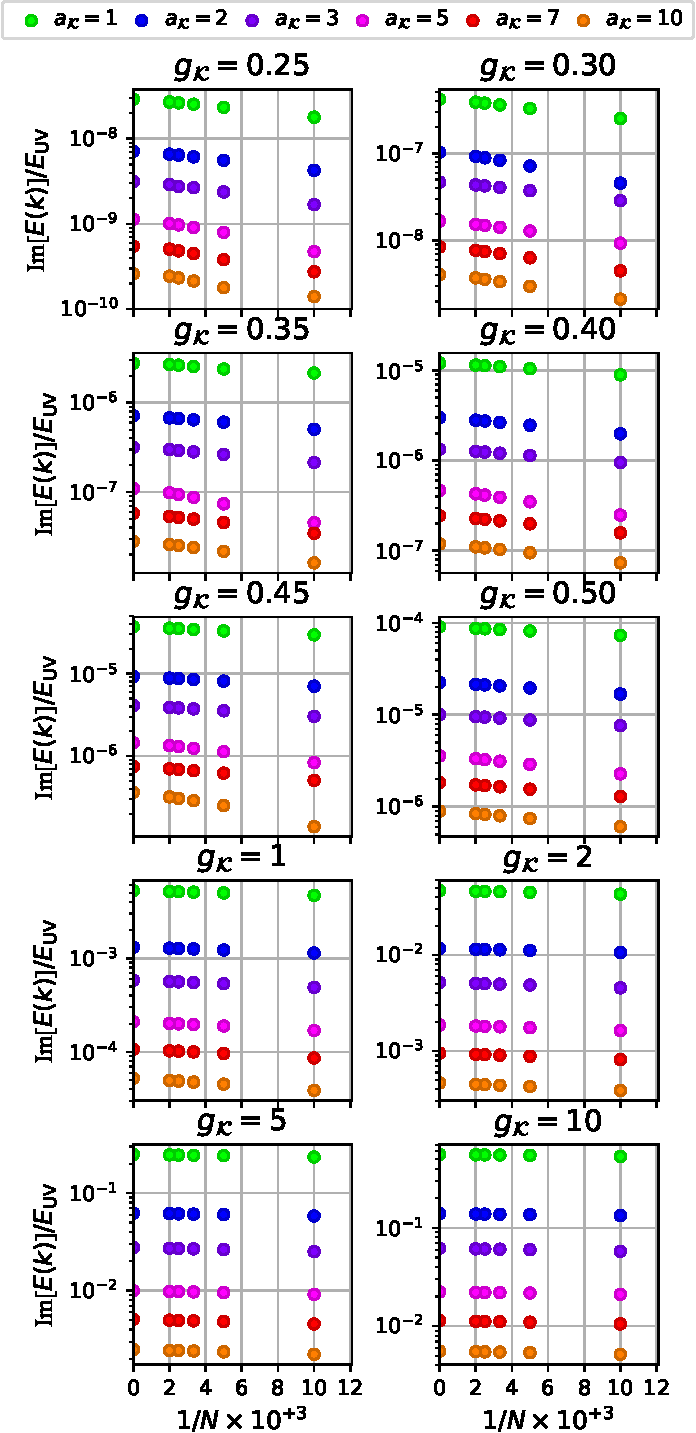
\includegraphics[scale=0.6]{./PlotReport/PlotsSizesL0}
\caption{Extrapolation of the imaginary parts in the channel $\ell=0$ as the linear regresion given in Eq. \eqref{eq:Zero-Ansatz} for five different system sizes $N=$ 100, 200, 300, 400 and 500. The infinite-size limits are listed with their standard errors in Tab. \ref{tab:Inf-size-points-L0}. }
\end{figure}

\begin{table}
\begin{tabular}{ccc}
%\multicolumn{3}{c}{$\ell=0$}	\\ \hline \hline 
$a_{\mathcal{K}}$	&	$1/g_{\mathcal{K}}$	&	
$\mathrm{Im}[E^{(0)}](a_{\mathcal{K}},g_{\mathcal{K}})$	\\ \hline \hline 
$ 1 $ & $ 4.      $ & $ (2.92152\pm0.00789)\times 10^{-8}$ \\
$ 1 $ & $ 3.33333 $ & $ (4.16824\pm0.03815)\times 10^{-7}$ \\
$ 1 $ & $ 2.85714 $ & $ (2.78958\pm0.04014)\times 10^{-6}$ \\
$ 1 $ & $ 2.5     $ & $ (1.20918\pm0.00247)\times 10^{-5}$ \\
$ 1 $ & $ 2.22222 $ & $ (3.67784\pm0.13941)\times 10^{-6}$ \\
$ 1 $ & $ 2.      $ & $ (9.05161\pm0.11104)\times 10^{-6}$ \\ \hline \hline 
$ 2 $ & $ 4.      $ & $ (7.13223\pm0.05980)\times 10^{-9}$ \\
$ 2 $ & $ 3.33333 $ & $ (1.02927\pm0.01370)\times 10^{-7}$ \\
$ 2 $ & $ 2.85714 $ & $ (7.17900\pm0.02154)\times 10^{-7}$ \\
$ 2 $ & $ 2.5     $ & $ (2.99848\pm0.01200)\times 10^{-6}$ \\
$ 2 $ & $ 2.22222 $ & $ (9.23142\pm0.01736)\times 10^{-6}$ \\
$ 2 $ & $ 2.      $ & $ (2.25623\pm0.04265)\times 10^{-6}$ \\ \hline \hline 
$ 3 $ & $ 4.      $ & $ (3.15043\pm0.03078)\times 10^{-9}$ \\
$ 3 $ & $ 3.33333 $ & $ (4.68115\pm0.02323)\times 10^{-8}$ \\
$ 3 $ & $ 2.85714 $ & $ (3.18026\pm0.01185)\times 10^{-7}$ \\
$ 3 $ & $ 2.5     $ & $ (1.33870\pm0.00375)\times 10^{-6}$ \\
$ 3 $ & $ 2.22222 $ & $ (4.09552\pm0.00318)\times 10^{-6}$ \\
$ 3 $ & $ 2.      $ & $ (1.00257\pm0.01928)\times 10^{-6}$ \\ \hline \hline 
$ 5 $ & $ 4.      $ & $ (1.13815\pm0.00536)\times 10^{-9}$ \\
$ 5 $ & $ 3.33333 $ & $ (1.67524\pm0.00993)\times 10^{-8}$ \\
$ 5 $ & $ 2.85714 $ & $ (1.09754\pm0.01789)\times 10^{-7}$ \\
$ 5 $ & $ 2.5     $ & $ (4.67946\pm0.04882)\times 10^{-7}$ \\
$ 5 $ & $ 2.22222 $ & $ (1.45688\pm0.00646)\times 10^{-6}$ \\
$ 5 $ & $ 2.      $ & $ (3.56892\pm0.01652)\times 10^{-6}$ \\ \hline \hline 
$ 7 $ & $ 4.      $ & $ (5.48481\pm0.15749)\times 10^{-10}$ \\
$ 7 $ & $ 3.33333 $ & $ (8.46152\pm0.07365)\times 10^{-9}$ \\
$ 7 $ & $ 2.85714 $ & $ (5.79094\pm0.03126)\times 10^{-8}$ \\
$ 7 $ & $ 2.5     $ & $ (2.44125\pm0.01064)\times 10^{-7}$ \\
$ 7 $ & $ 2.22222 $ & $ (7.47993\pm0.02632)\times 10^{-7}$ \\
$ 7 $ & $ 2.      $ & $ (1.83301\pm0.00538)\times 10^{-6}$ \\ \hline \hline 
$10 $ & $ 4.      $ & $ (2.59171\pm0.10806)\times 10^{-10}$ \\
$10 $ & $ 3.33333 $ & $ (4.06583\pm0.05989)\times 10^{-9}$ \\
$10 $ & $ 2.85714 $ & $ (2.81035\pm0.02282)\times 10^{-8}$ \\
$10 $ & $ 2.5     $ & $ (1.19031\pm0.00658)\times 10^{-7}$ \\
$10 $ & $ 2.22222 $ & $ (3.64543\pm0.00559)\times 10^{-7}$ \\
$10 $ & $ 2.      $ & $ (8.95646\pm0.03185)\times 10^{-7}$ \\ \hline \hline  
\end{tabular}
\caption{Infinite-size limits $\mathrm{Im}[E^{(0)}](a_{\mathcal{K}},g_{\mathcal{K}})$ of the points on the plane $a_{\mathcal{K}}$ vs. $1/g_{\mathcal{K}}$ extrapolated using least-squares on the Eq. \eqref{eq:Zero-Ansatz} for the channel $\ell=0$.}
\label{tab:Inf-size-points-L0}
\end{table}

Lorem ipsum dolor sit amet, consectetur adipiscing elit. Quisque eu pharetra ligula, in scelerisque risus. Mauris convallis neque elit, at tincidunt lectus venenatis et. Donec ultricies eros nec nisl posuere, vitae scelerisque enim fringilla. Maecenas eget odio dapibus, egestas ante a, tempor neque. Nullam in nisi varius, laoreet urna sit amet, hendrerit erat. Maecenas id ligula posuere, tincidunt nisi a, scelerisque libero. Quisque maximus quis sem eleifend fermentum. Ut pharetra dui quis pharetra consectetur. Pellentesque commodo lacinia urna. Aliquam nibh nulla, facilisis id cursus eget, tristique non neque.





\begin{figure}
\centering 
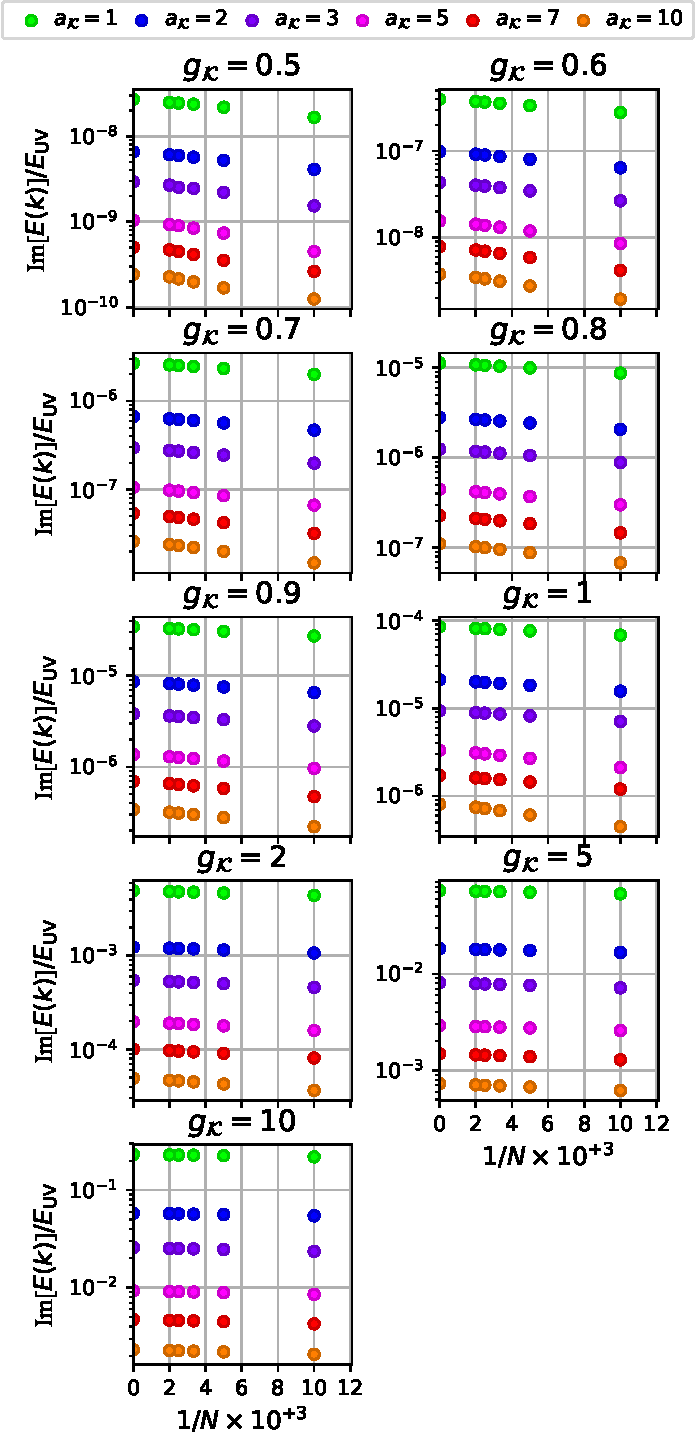
\includegraphics[scale=0.6]{./PlotReport/PlotsSizesL2}
\caption{Extrapolation of the imaginary parts in the channel $\ell=2$ as the linear regresion given in Eq. \eqref{eq:Zero-Ansatz} for five different system sizes $N=$ 100, 200, 300, 400 and 500. The infinite-size limits are listed with their standard errors in Tab. \ref{tab:Inf-size-points-L2}. }
\end{figure}


\begin{table}
\begin{tabular}{ccc}
\multicolumn{3}{c}{$\ell=2$}	\\ \hline \hline 
$a_{\mathcal{K}}$	&	$1/g_{\mathcal{K}}$	&	
$\mathrm{Im}[E^{(2)}](a_{\mathcal{K}},g_{\mathcal{K}})$	\\ \hline \hline 
    $ 1 $ & $ 2.      $ & $ (2.71270\pm 0.00588)\times 10^{-8} $ \\
    $ 1 $ & $ 1.66667 $ & $ (3.95448\pm 0.01197)\times 10^{-7} $ \\
    $ 1 $ & $ 1.42857 $ & $ (2.68217\pm 0.00584)\times 10^{-6} $ \\
    $ 1 $ & $ 1.25    $ & $ (1.12794\pm 0.00193)\times 10^{-5} $ \\
    $ 1 $ & $ 1.11111 $ & $ (3.45039\pm 0.00493)\times 10^{-5} $ \\ \hline \hline  
    $ 2 $ & $ 2.      $ & $ (6.55098\pm 0.05278)\times 10^{-9} $ \\
    $ 2 $ & $ 1.66667 $ & $ (9.81992\pm 0.04536)\times 10^{-8} $ \\
    $ 2 $ & $ 1.42857 $ & $ (6.67918\pm 0.02030)\times 10^{-7} $ \\
    $ 2 $ & $ 1.25    $ & $ (2.81190\pm 0.00656)\times 10^{-6} $ \\
    $ 2 $ & $ 1.11111 $ & $ (8.60731\pm 0.01642)\times 10^{-6} $ \\ \hline \hline  
    $ 3 $ & $ 2.      $ & $ (2.92241\pm 0.02954)\times 10^{-9} $ \\
    $ 3 $ & $ 1.66667 $ & $ (4.34776\pm 0.02244)\times 10^{-8} $ \\
    $ 3 $ & $ 1.42857 $ & $ (2.95870\pm 0.01117)\times 10^{-7} $ \\
    $ 3 $ & $ 1.25    $ & $ (1.24681\pm 0.00355)\times 10^{-6} $ \\
    $ 3 $ & $ 1.11111 $ & $ (3.81851\pm 0.00882)\times 10^{-6} $ \\ \hline \hline  
    $ 5 $ & $ 2.      $ & $ (1.04595\pm 0.00465)\times 10^{-9} $ \\
    $ 5 $ & $ 1.66667 $ & $ (1.55836\pm 0.00861)\times 10^{-8} $ \\
    $ 5 $ & $ 1.42857 $ & $ (1.05890\pm 0.00543)\times 10^{-7} $ \\
    $ 5 $ & $ 1.25    $ & $ (4.47072\pm 0.01660)\times 10^{-7} $ \\
    $ 5 $ & $ 1.11111 $ & $ (1.37043\pm 0.00409)\times 10^{-6} $ \\ \hline \hline  
    $ 7 $ & $ 2.      $ & $ (5.05321\pm 0.15138)\times 10^{-10} $ \\
    $ 7 $ & $ 1.66667 $ & $ (7.84517\pm 0.07565)\times 10^{-9} $ \\
    $ 7 $ & $ 1.42857 $ & $ (5.38602\pm 0.02976)\times 10^{-8} $ \\
    $ 7 $ & $ 1.25    $ & $ (2.27356\pm 0.01000)\times 10^{-7} $ \\
    $ 7 $ & $ 1.11111 $ & $ (6.97338\pm 0.02489\times 10^{-7} $ \\ \hline \hline  
    $10 $ & $ 2.      $ & $ (2.42989\pm 0.08010\times 10^{-10} $ \\
    $10 $ & $ 1.66667 $ & $ (3.78447\pm 0.05330\times 10^{-9} $ \\
    $10 $ & $ 1.42857 $ & $ (2.61431\pm 0.02132\times 10^{-8} $ \\
    $10 $ & $ 1.25    $ & $ (1.10834\pm 0.00624\times 10^{-7} $ \\
    $10 $ & $ 1.11111 $ & $ (3.40468\pm 0.01489\times 10^{-7} $ \\ \hline \hline  
\end{tabular}
\caption{Infinite-size limits $\mathrm{Im}[E^{(2)}](a_{\mathcal{K}},g_{\mathcal{K}})$ of the points on the plane $a_{\mathcal{K}}$ vs. $1/g_{\mathcal{K}}$ extrapolated using least-squares on the Eq. \eqref{eq:Zero-Ansatz} for the channel $\ell=2$.}
\label{tab:Inf-size-points-L2}
\end{table}


Proin risus sem, viverra vitae ornare ut, imperdiet a erat. Ut aliquet lorem sit amet elit efficitur auctor. Praesent consequat magna a neque feugiat, eget facilisis sem eleifend. Proin id posuere est, nec sodales nibh. Maecenas lacus felis, fringilla eu ligula at, gravida feugiat orci. In id faucibus massa. Phasellus iaculis iaculis mauris, vitae congue orci hendrerit eu. Proin interdum nisl at justo scelerisque ullamcorper. Maecenas tincidunt lectus quis gravida faucibus. Vestibulum tempor fermentum egestas.

Proin vitae semper dolor. Etiam diam ex, lobortis vitae rutrum sed, tempus at diam. Nunc ut felis mauris. Duis suscipit dui eu enim cursus, aliquet consequat est bibendum. Maecenas id enim consectetur, iaculis purus ac, consectetur quam. Suspendisse vel interdum turpis. Duis hendrerit tempor lacus, eu iaculis orci congue eu. Nam vitae tellus non nisi euismod feugiat vitae vitae ex. Quisque felis mauris, pulvinar sed dui sit amet, facilisis ultricies tortor. Quisque nibh massa, malesuada quis nisl sodales, faucibus semper ligula.

Duis imperdiet massa eu lacus fringilla, et pulvinar eros dapibus. Etiam dictum vulputate tempus. Integer felis dolor, mattis in tincidunt eu, sodales ac orci. Curabitur fermentum aliquam finibus. Praesent non dui nunc. Ut commodo vulputate lorem, nec pretium nisi lacinia vitae. Donec fermentum elementum ex vel mollis. Donec turpis nisi, placerat vel sollicitudin in, bibendum vel ipsum. Aliquam venenatis non nisl ut rutrum. Cras sed est tincidunt elit euismod fermentum et quis nisi. Ut fringilla ligula nisl, sed lobortis nunc laoreet et.

Morbi arcu leo, auctor ut luctus eu, eleifend sed lorem. Sed commodo molestie ligula ut tempor. Aenean posuere vel velit et ullamcorper. Integer consectetur semper arcu non hendrerit. Suspendisse ornare leo vel ornare sollicitudin. Vivamus elementum lacinia turpis quis suscipit. Duis varius aliquam tortor. Vestibulum ante ipsum primis in faucibus orci luctus et ultrices posuere cubilia curae; Morbi a tristique mauris. Quisque pretium, nibh in ornare elementum, neque velit efficitur dui, nec fermentum ipsum risus sit amet magna. Donec elit quam, cursus sed mollis non, aliquam vitae felis.




















\begin{comment}
\begin{thebibliography}{10}

\bibitem{giamarchi2003quantum}
T.~Giamarchi, {\em Quantum physics in one dimension}, vol.~121.
\newblock Clarendon press, 2003.

\bibitem{luther1979tomonaga}
A.~Luther, ``Tomonaga fermions and the dirac equation in three dimensions,''
  {\em Physical Review B}, vol.~19, no.~1, p.~320, 1979.

\bibitem{haldane2005luttinger}
F.~Haldane, ``Luttinger's theorem and bosonization of the fermi surface,'' {\em
  arXiv preprint cond-mat/0505529}, 2005.

\bibitem{houghton1993bosonization}
A.~Houghton and J. B. ~Marston, ``Bosonization and fermion liquids in dimensions
  greater than one,'' {\em Physical Review B}, vol.~48, no.~11, p.~7790, 1993.

\bibitem{neto1994bosonization}
A. H. Castro Neto and E.~Fradkin, ``Bosonization of the low energy excitations of
  fermi liquids,'' {\em Physical review letters}, vol.~72, no.~10, p.~1393,
  1994.

\bibitem{houghton2000multidimensional}
A.~Houghton, H.-J. Kwon, and J.~Marston, ``Multidimensional bosonization,''
  {\em Advances in Physics}, vol.~49, no.~2, pp.~141--228, 2000.

\bibitem{neto1995exact}
A. H. Castro Neto and E. H.~Fradkin, ``Exact solution of the landau fixed point via
  bosonization,'' {\em Physical Review B}, vol.~51, no.~7, p.~4084, 1995.

\bibitem{baym1961conservation}
G.~Baym and L.~P. Kadanoff, ``Conservation laws and correlation functions,''
  {\em Physical Review}, vol.~124, no.~2, p.~287, 1961.

\bibitem{PhysRev.127.1391}
G.~Baym, ``Self-consistent approximations in many-body systems,'' {\em Phys.
  Rev.}, vol.~127, pp.~1391--1401, Aug 1962.

\bibitem{PhysRevB.50.7526}
A.~W.~W. Ludwig, M.~P.~A. Fisher, R.~Shankar, and G.~Grinstein, ``Integer
  quantum hall transition: An alternative approach and exact results,'' {\em
  Phys. Rev. B}, vol.~50, pp.~7526--7552, Sep 1994.

\bibitem{ando2002dynamical}
T.~Ando, Y.~Zheng, and H.~Suzuura, ``Dynamical conductivity and zero-mode
  anomaly in honeycomb lattices,'' {\em Journal of the Physical Society of
  Japan}, vol.~71, no.~5, pp.~1318--1324, 2002.

\bibitem{mishchenko2008minimal}
E.~Mishchenko, ``Minimal conductivity in graphene: Interaction corrections and
  ultraviolet anomaly,'' {\em EPL (Europhysics Letters)}, vol.~83, no.~1,
  p.~17005, 2008.

\bibitem{herbut2008coulomb}
I.~F. Herbut, V.~Juri{\v{c}}i{\'c}, and O.~Vafek, ``Coulomb interaction,
  ripples, and the minimal conductivity of graphene,'' {\em Physical review
  letters}, vol.~100, no.~4, p.~046403, 2008.

\bibitem{sheehy2009optical}
D.~E. Sheehy and J.~Schmalian, ``Optical transparency of graphene as determined
  by the fine-structure constant,'' {\em Physical Review B}, vol.~80, no.~19,
  p.~193411, 2009.

\bibitem{abedinpour2011drude}
S.~H. Abedinpour, G.~Vignale, A.~Principi, M.~Polini, W.-K. Tse, and A.~H.
  MacDonald, ``Drude weight, plasmon dispersion, and ac conductivity in doped
  graphene sheets,'' {\em Physical Review B}, vol.~84, no.~4, p.~045429, 2011.

\bibitem{sodemann2012interaction}
I.~Sodemann and M.~M. Fogler, ``Interaction corrections to the polarization
  function of graphene,'' {\em Physical Review B}, vol.~86, no.~11, p.~115408,
  2012.

\bibitem{gazzola2013conductivity}
G.~Gazzola, A.~Cherchiglia, L.~Cabral, M.~Nemes, and M.~Sampaio, ``Conductivity
  of coulomb interacting massless dirac particles in graphene:
  Regularization-dependent parameters and symmetry constraints,'' {\em EPL
  (Europhysics Letters)}, vol.~104, no.~2, p.~27002, 2013.

\bibitem{barnes2014effective}
E.~Barnes, E. H. ~Hwang, R. E. ~Throckmorton, and S. Das Sarma, ``Effective field
  theory, three-loop perturbative expansion, and their experimental
  implications in graphene many-body effects,'' {\em Physical Review B},
  vol.~89, no.~23, p.~235431, 2014.

\bibitem{teber2014interaction}
S.~Teber and A.~Kotikov, ``Interaction corrections to the minimal conductivity
  of graphene via dimensional regularization,'' {\em EPL (Europhysics
  Letters)}, vol.~107, no.~5, p.~57001, 2014.

\bibitem{teber2018field}
S.~Teber and A.~Kotikov, ``Field theoretic renormalization study of interaction
  corrections to the universal ac conductivity of graphene,'' {\em Journal of
  High Energy Physics}, vol.~2018, no.~7, p.~82, 2018.

\bibitem{boyda2016many}
D. L.~Boyda, V. V.~Braguta, M. I.~Katsnelson, and M. V.~Ulybyshev, ``Many-body effects on
  graphene conductivity: Quantum monte carlo calculations,'' {\em Physical
  Review B}, vol.~94, no.~8, p.~085421, 2016.

\bibitem{li2008dirac}
Z.~Li, E.~A. Henriksen, Z.~Jiang, Z.~Hao, M.~C. Martin, P.~Kim, H.~Stormer, and
  D.~N. Basov, ``Dirac charge dynamics in graphene by infrared spectroscopy,''
  {\em Nature Physics}, vol.~4, no.~7, p.~532, 2008.

\bibitem{mak2008measurement}
K.~F. Mak, M.~Y. Sfeir, Y.~Wu, C.~H. Lui, J.~A. Misewich, and T.~F. Heinz,
  ``Measurement of the optical conductivity of graphene,'' {\em Physical review
  letters}, vol.~101, no.~19, p.~196405, 2008.

\bibitem{nair2008fine}
R.~R. Nair, P.~Blake, A.~N. Grigorenko, K.~S. Novoselov, T.~J. Booth,
  T.~Stauber, N.~M. Peres, and A.~K. Geim, ``Fine structure constant defines
  visual transparency of graphene,'' {\em Science}, vol.~320, no.~5881,
  pp.~1308--1308, 2008.

\bibitem{auerbach2012interacting}
A.~Auerbach, {\em Interacting electrons and quantum magnetism}.
\newblock Springer Science \& Business Media, 2012.

\bibitem{SupplementalMaterial}
See the supplemental material for derivations of the expressions.

\bibitem{vanHemmen1980note}
J.~Van~Hemmen, ``A note on the diagonalization of quadratic boson and fermion
  hamiltonians,'' {\em Zeitschrift f{\"u}r Physik B Condensed Matter}, vol.~38,
  no.~3, pp.~271--277, 1980.

\bibitem{armitage2018weyl}
N. P.~Armitage, E. J.~Mele, and A.~Vishwanath, ``Weyl and dirac semimetals in
  three-dimensional solids,'' {\em Reviews of Modern Physics}, vol.~90, no.~1,
  p.~015001, 2018.

\bibitem{bradlyn2016beyond}
B.~Bradlyn, J.~Cano, Z.~Wang, M.~Vergniory, C.~Felser, R.~J. Cava, and B.~A.
  Bernevig, ``Beyond dirac and weyl fermions: Unconventional quasiparticles in
  conventional crystals,'' {\em Science}, vol.~353, no.~6299, p.~aaf5037, 2016.

\end{thebibliography}
\end{comment}

%\bibliography{Manuscript}
%\bibliographystyle{ieeetr}

\end{document} 
